\documentclass[10pt]{article} % For LaTeX2e
\usepackage{tmlr}
% If accepted, instead use the following line for the camera-ready submission:
%\usepackage[accepted]{tmlr}
% To de-anonymize and remove mentions to TMLR (for example for posting to preprint servers), instead use the following:
%\usepackage[preprint]{tmlr}

% Optional math commands from https://github.com/goodfeli/dlbook_notation.
%%%%% NEW MATH DEFINITIONS %%%%%

\usepackage{amsmath,amsfonts,bm}

% Mark sections of captions for referring to divisions of figures
\newcommand{\figleft}{{\em (Left)}}
\newcommand{\figcenter}{{\em (Center)}}
\newcommand{\figright}{{\em (Right)}}
\newcommand{\figtop}{{\em (Top)}}
\newcommand{\figbottom}{{\em (Bottom)}}
\newcommand{\captiona}{{\em (a)}}
\newcommand{\captionb}{{\em (b)}}
\newcommand{\captionc}{{\em (c)}}
\newcommand{\captiond}{{\em (d)}}

% Highlight a newly defined term
\newcommand{\newterm}[1]{{\bf #1}}


% Figure reference, lower-case.
\def\figref#1{figure~\ref{#1}}
% Figure reference, capital. For start of sentence
\def\Figref#1{Figure~\ref{#1}}
\def\twofigref#1#2{figures \ref{#1} and \ref{#2}}
\def\quadfigref#1#2#3#4{figures \ref{#1}, \ref{#2}, \ref{#3} and \ref{#4}}
% Section reference, lower-case.
\def\secref#1{section~\ref{#1}}
% Section reference, capital.
\def\Secref#1{Section~\ref{#1}}
% Reference to two sections.
\def\twosecrefs#1#2{sections \ref{#1} and \ref{#2}}
% Reference to three sections.
\def\secrefs#1#2#3{sections \ref{#1}, \ref{#2} and \ref{#3}}
% Reference to an equation, lower-case.
\def\eqref#1{equation~\ref{#1}}
% Reference to an equation, upper case
\def\Eqref#1{Equation~\ref{#1}}
% A raw reference to an equation---avoid using if possible
\def\plaineqref#1{\ref{#1}}
% Reference to a chapter, lower-case.
\def\chapref#1{chapter~\ref{#1}}
% Reference to an equation, upper case.
\def\Chapref#1{Chapter~\ref{#1}}
% Reference to a range of chapters
\def\rangechapref#1#2{chapters\ref{#1}--\ref{#2}}
% Reference to an algorithm, lower-case.
\def\algref#1{algorithm~\ref{#1}}
% Reference to an algorithm, upper case.
\def\Algref#1{Algorithm~\ref{#1}}
\def\twoalgref#1#2{algorithms \ref{#1} and \ref{#2}}
\def\Twoalgref#1#2{Algorithms \ref{#1} and \ref{#2}}
% Reference to a part, lower case
\def\partref#1{part~\ref{#1}}
% Reference to a part, upper case
\def\Partref#1{Part~\ref{#1}}
\def\twopartref#1#2{parts \ref{#1} and \ref{#2}}

\def\ceil#1{\lceil #1 \rceil}
\def\floor#1{\lfloor #1 \rfloor}
\def\1{\bm{1}}
\newcommand{\train}{\mathcal{D}}
\newcommand{\valid}{\mathcal{D_{\mathrm{valid}}}}
\newcommand{\test}{\mathcal{D_{\mathrm{test}}}}

\def\eps{{\epsilon}}


% Random variables
\def\reta{{\textnormal{$\eta$}}}
\def\ra{{\textnormal{a}}}
\def\rb{{\textnormal{b}}}
\def\rc{{\textnormal{c}}}
\def\rd{{\textnormal{d}}}
\def\re{{\textnormal{e}}}
\def\rf{{\textnormal{f}}}
\def\rg{{\textnormal{g}}}
\def\rh{{\textnormal{h}}}
\def\ri{{\textnormal{i}}}
\def\rj{{\textnormal{j}}}
\def\rk{{\textnormal{k}}}
\def\rl{{\textnormal{l}}}
% rm is already a command, just don't name any random variables m
\def\rn{{\textnormal{n}}}
\def\ro{{\textnormal{o}}}
\def\rp{{\textnormal{p}}}
\def\rq{{\textnormal{q}}}
\def\rr{{\textnormal{r}}}
\def\rs{{\textnormal{s}}}
\def\rt{{\textnormal{t}}}
\def\ru{{\textnormal{u}}}
\def\rv{{\textnormal{v}}}
\def\rw{{\textnormal{w}}}
\def\rx{{\textnormal{x}}}
\def\ry{{\textnormal{y}}}
\def\rz{{\textnormal{z}}}

% Random vectors
\def\rvepsilon{{\mathbf{\epsilon}}}
\def\rvtheta{{\mathbf{\theta}}}
\def\rva{{\mathbf{a}}}
\def\rvb{{\mathbf{b}}}
\def\rvc{{\mathbf{c}}}
\def\rvd{{\mathbf{d}}}
\def\rve{{\mathbf{e}}}
\def\rvf{{\mathbf{f}}}
\def\rvg{{\mathbf{g}}}
\def\rvh{{\mathbf{h}}}
\def\rvu{{\mathbf{i}}}
\def\rvj{{\mathbf{j}}}
\def\rvk{{\mathbf{k}}}
\def\rvl{{\mathbf{l}}}
\def\rvm{{\mathbf{m}}}
\def\rvn{{\mathbf{n}}}
\def\rvo{{\mathbf{o}}}
\def\rvp{{\mathbf{p}}}
\def\rvq{{\mathbf{q}}}
\def\rvr{{\mathbf{r}}}
\def\rvs{{\mathbf{s}}}
\def\rvt{{\mathbf{t}}}
\def\rvu{{\mathbf{u}}}
\def\rvv{{\mathbf{v}}}
\def\rvw{{\mathbf{w}}}
\def\rvx{{\mathbf{x}}}
\def\rvy{{\mathbf{y}}}
\def\rvz{{\mathbf{z}}}

% Elements of random vectors
\def\erva{{\textnormal{a}}}
\def\ervb{{\textnormal{b}}}
\def\ervc{{\textnormal{c}}}
\def\ervd{{\textnormal{d}}}
\def\erve{{\textnormal{e}}}
\def\ervf{{\textnormal{f}}}
\def\ervg{{\textnormal{g}}}
\def\ervh{{\textnormal{h}}}
\def\ervi{{\textnormal{i}}}
\def\ervj{{\textnormal{j}}}
\def\ervk{{\textnormal{k}}}
\def\ervl{{\textnormal{l}}}
\def\ervm{{\textnormal{m}}}
\def\ervn{{\textnormal{n}}}
\def\ervo{{\textnormal{o}}}
\def\ervp{{\textnormal{p}}}
\def\ervq{{\textnormal{q}}}
\def\ervr{{\textnormal{r}}}
\def\ervs{{\textnormal{s}}}
\def\ervt{{\textnormal{t}}}
\def\ervu{{\textnormal{u}}}
\def\ervv{{\textnormal{v}}}
\def\ervw{{\textnormal{w}}}
\def\ervx{{\textnormal{x}}}
\def\ervy{{\textnormal{y}}}
\def\ervz{{\textnormal{z}}}

% Random matrices
\def\rmA{{\mathbf{A}}}
\def\rmB{{\mathbf{B}}}
\def\rmC{{\mathbf{C}}}
\def\rmD{{\mathbf{D}}}
\def\rmE{{\mathbf{E}}}
\def\rmF{{\mathbf{F}}}
\def\rmG{{\mathbf{G}}}
\def\rmH{{\mathbf{H}}}
\def\rmI{{\mathbf{I}}}
\def\rmJ{{\mathbf{J}}}
\def\rmK{{\mathbf{K}}}
\def\rmL{{\mathbf{L}}}
\def\rmM{{\mathbf{M}}}
\def\rmN{{\mathbf{N}}}
\def\rmO{{\mathbf{O}}}
\def\rmP{{\mathbf{P}}}
\def\rmQ{{\mathbf{Q}}}
\def\rmR{{\mathbf{R}}}
\def\rmS{{\mathbf{S}}}
\def\rmT{{\mathbf{T}}}
\def\rmU{{\mathbf{U}}}
\def\rmV{{\mathbf{V}}}
\def\rmW{{\mathbf{W}}}
\def\rmX{{\mathbf{X}}}
\def\rmY{{\mathbf{Y}}}
\def\rmZ{{\mathbf{Z}}}

% Elements of random matrices
\def\ermA{{\textnormal{A}}}
\def\ermB{{\textnormal{B}}}
\def\ermC{{\textnormal{C}}}
\def\ermD{{\textnormal{D}}}
\def\ermE{{\textnormal{E}}}
\def\ermF{{\textnormal{F}}}
\def\ermG{{\textnormal{G}}}
\def\ermH{{\textnormal{H}}}
\def\ermI{{\textnormal{I}}}
\def\ermJ{{\textnormal{J}}}
\def\ermK{{\textnormal{K}}}
\def\ermL{{\textnormal{L}}}
\def\ermM{{\textnormal{M}}}
\def\ermN{{\textnormal{N}}}
\def\ermO{{\textnormal{O}}}
\def\ermP{{\textnormal{P}}}
\def\ermQ{{\textnormal{Q}}}
\def\ermR{{\textnormal{R}}}
\def\ermS{{\textnormal{S}}}
\def\ermT{{\textnormal{T}}}
\def\ermU{{\textnormal{U}}}
\def\ermV{{\textnormal{V}}}
\def\ermW{{\textnormal{W}}}
\def\ermX{{\textnormal{X}}}
\def\ermY{{\textnormal{Y}}}
\def\ermZ{{\textnormal{Z}}}

% Vectors
\def\vzero{{\bm{0}}}
\def\vone{{\bm{1}}}
\def\vmu{{\bm{\mu}}}
\def\vtheta{{\bm{\theta}}}
\def\va{{\bm{a}}}
\def\vb{{\bm{b}}}
\def\vc{{\bm{c}}}
\def\vd{{\bm{d}}}
\def\ve{{\bm{e}}}
\def\vf{{\bm{f}}}
\def\vg{{\bm{g}}}
\def\vh{{\bm{h}}}
\def\vi{{\bm{i}}}
\def\vj{{\bm{j}}}
\def\vk{{\bm{k}}}
\def\vl{{\bm{l}}}
\def\vm{{\bm{m}}}
\def\vn{{\bm{n}}}
\def\vo{{\bm{o}}}
\def\vp{{\bm{p}}}
\def\vq{{\bm{q}}}
\def\vr{{\bm{r}}}
\def\vs{{\bm{s}}}
\def\vt{{\bm{t}}}
\def\vu{{\bm{u}}}
\def\vv{{\bm{v}}}
\def\vw{{\bm{w}}}
\def\vx{{\bm{x}}}
\def\vy{{\bm{y}}}
\def\vz{{\bm{z}}}

% Elements of vectors
\def\evalpha{{\alpha}}
\def\evbeta{{\beta}}
\def\evepsilon{{\epsilon}}
\def\evlambda{{\lambda}}
\def\evomega{{\omega}}
\def\evmu{{\mu}}
\def\evpsi{{\psi}}
\def\evsigma{{\sigma}}
\def\evtheta{{\theta}}
\def\eva{{a}}
\def\evb{{b}}
\def\evc{{c}}
\def\evd{{d}}
\def\eve{{e}}
\def\evf{{f}}
\def\evg{{g}}
\def\evh{{h}}
\def\evi{{i}}
\def\evj{{j}}
\def\evk{{k}}
\def\evl{{l}}
\def\evm{{m}}
\def\evn{{n}}
\def\evo{{o}}
\def\evp{{p}}
\def\evq{{q}}
\def\evr{{r}}
\def\evs{{s}}
\def\evt{{t}}
\def\evu{{u}}
\def\evv{{v}}
\def\evw{{w}}
\def\evx{{x}}
\def\evy{{y}}
\def\evz{{z}}

% Matrix
\def\mA{{\bm{A}}}
\def\mB{{\bm{B}}}
\def\mC{{\bm{C}}}
\def\mD{{\bm{D}}}
\def\mE{{\bm{E}}}
\def\mF{{\bm{F}}}
\def\mG{{\bm{G}}}
\def\mH{{\bm{H}}}
\def\mI{{\bm{I}}}
\def\mJ{{\bm{J}}}
\def\mK{{\bm{K}}}
\def\mL{{\bm{L}}}
\def\mM{{\bm{M}}}
\def\mN{{\bm{N}}}
\def\mO{{\bm{O}}}
\def\mP{{\bm{P}}}
\def\mQ{{\bm{Q}}}
\def\mR{{\bm{R}}}
\def\mS{{\bm{S}}}
\def\mT{{\bm{T}}}
\def\mU{{\bm{U}}}
\def\mV{{\bm{V}}}
\def\mW{{\bm{W}}}
\def\mX{{\bm{X}}}
\def\mY{{\bm{Y}}}
\def\mZ{{\bm{Z}}}
\def\mBeta{{\bm{\beta}}}
\def\mPhi{{\bm{\Phi}}}
\def\mLambda{{\bm{\Lambda}}}
\def\mSigma{{\bm{\Sigma}}}

% Tensor
\DeclareMathAlphabet{\mathsfit}{\encodingdefault}{\sfdefault}{m}{sl}
\SetMathAlphabet{\mathsfit}{bold}{\encodingdefault}{\sfdefault}{bx}{n}
\newcommand{\tens}[1]{\bm{\mathsfit{#1}}}
\def\tA{{\tens{A}}}
\def\tB{{\tens{B}}}
\def\tC{{\tens{C}}}
\def\tD{{\tens{D}}}
\def\tE{{\tens{E}}}
\def\tF{{\tens{F}}}
\def\tG{{\tens{G}}}
\def\tH{{\tens{H}}}
\def\tI{{\tens{I}}}
\def\tJ{{\tens{J}}}
\def\tK{{\tens{K}}}
\def\tL{{\tens{L}}}
\def\tM{{\tens{M}}}
\def\tN{{\tens{N}}}
\def\tO{{\tens{O}}}
\def\tP{{\tens{P}}}
\def\tQ{{\tens{Q}}}
\def\tR{{\tens{R}}}
\def\tS{{\tens{S}}}
\def\tT{{\tens{T}}}
\def\tU{{\tens{U}}}
\def\tV{{\tens{V}}}
\def\tW{{\tens{W}}}
\def\tX{{\tens{X}}}
\def\tY{{\tens{Y}}}
\def\tZ{{\tens{Z}}}


% Graph
\def\gA{{\mathcal{A}}}
\def\gB{{\mathcal{B}}}
\def\gC{{\mathcal{C}}}
\def\gD{{\mathcal{D}}}
\def\gE{{\mathcal{E}}}
\def\gF{{\mathcal{F}}}
\def\gG{{\mathcal{G}}}
\def\gH{{\mathcal{H}}}
\def\gI{{\mathcal{I}}}
\def\gJ{{\mathcal{J}}}
\def\gK{{\mathcal{K}}}
\def\gL{{\mathcal{L}}}
\def\gM{{\mathcal{M}}}
\def\gN{{\mathcal{N}}}
\def\gO{{\mathcal{O}}}
\def\gP{{\mathcal{P}}}
\def\gQ{{\mathcal{Q}}}
\def\gR{{\mathcal{R}}}
\def\gS{{\mathcal{S}}}
\def\gT{{\mathcal{T}}}
\def\gU{{\mathcal{U}}}
\def\gV{{\mathcal{V}}}
\def\gW{{\mathcal{W}}}
\def\gX{{\mathcal{X}}}
\def\gY{{\mathcal{Y}}}
\def\gZ{{\mathcal{Z}}}

% Sets
\def\sA{{\mathbb{A}}}
\def\sB{{\mathbb{B}}}
\def\sC{{\mathbb{C}}}
\def\sD{{\mathbb{D}}}
% Don't use a set called E, because this would be the same as our symbol
% for expectation.
\def\sF{{\mathbb{F}}}
\def\sG{{\mathbb{G}}}
\def\sH{{\mathbb{H}}}
\def\sI{{\mathbb{I}}}
\def\sJ{{\mathbb{J}}}
\def\sK{{\mathbb{K}}}
\def\sL{{\mathbb{L}}}
\def\sM{{\mathbb{M}}}
\def\sN{{\mathbb{N}}}
\def\sO{{\mathbb{O}}}
\def\sP{{\mathbb{P}}}
\def\sQ{{\mathbb{Q}}}
\def\sR{{\mathbb{R}}}
\def\sS{{\mathbb{S}}}
\def\sT{{\mathbb{T}}}
\def\sU{{\mathbb{U}}}
\def\sV{{\mathbb{V}}}
\def\sW{{\mathbb{W}}}
\def\sX{{\mathbb{X}}}
\def\sY{{\mathbb{Y}}}
\def\sZ{{\mathbb{Z}}}

% Entries of a matrix
\def\emLambda{{\Lambda}}
\def\emA{{A}}
\def\emB{{B}}
\def\emC{{C}}
\def\emD{{D}}
\def\emE{{E}}
\def\emF{{F}}
\def\emG{{G}}
\def\emH{{H}}
\def\emI{{I}}
\def\emJ{{J}}
\def\emK{{K}}
\def\emL{{L}}
\def\emM{{M}}
\def\emN{{N}}
\def\emO{{O}}
\def\emP{{P}}
\def\emQ{{Q}}
\def\emR{{R}}
\def\emS{{S}}
\def\emT{{T}}
\def\emU{{U}}
\def\emV{{V}}
\def\emW{{W}}
\def\emX{{X}}
\def\emY{{Y}}
\def\emZ{{Z}}
\def\emSigma{{\Sigma}}

% entries of a tensor
% Same font as tensor, without \bm wrapper
\newcommand{\etens}[1]{\mathsfit{#1}}
\def\etLambda{{\etens{\Lambda}}}
\def\etA{{\etens{A}}}
\def\etB{{\etens{B}}}
\def\etC{{\etens{C}}}
\def\etD{{\etens{D}}}
\def\etE{{\etens{E}}}
\def\etF{{\etens{F}}}
\def\etG{{\etens{G}}}
\def\etH{{\etens{H}}}
\def\etI{{\etens{I}}}
\def\etJ{{\etens{J}}}
\def\etK{{\etens{K}}}
\def\etL{{\etens{L}}}
\def\etM{{\etens{M}}}
\def\etN{{\etens{N}}}
\def\etO{{\etens{O}}}
\def\etP{{\etens{P}}}
\def\etQ{{\etens{Q}}}
\def\etR{{\etens{R}}}
\def\etS{{\etens{S}}}
\def\etT{{\etens{T}}}
\def\etU{{\etens{U}}}
\def\etV{{\etens{V}}}
\def\etW{{\etens{W}}}
\def\etX{{\etens{X}}}
\def\etY{{\etens{Y}}}
\def\etZ{{\etens{Z}}}

% The true underlying data generating distribution
\newcommand{\pdata}{p_{\rm{data}}}
% The empirical distribution defined by the training set
\newcommand{\ptrain}{\hat{p}_{\rm{data}}}
\newcommand{\Ptrain}{\hat{P}_{\rm{data}}}
% The model distribution
\newcommand{\pmodel}{p_{\rm{model}}}
\newcommand{\Pmodel}{P_{\rm{model}}}
\newcommand{\ptildemodel}{\tilde{p}_{\rm{model}}}
% Stochastic autoencoder distributions
\newcommand{\pencode}{p_{\rm{encoder}}}
\newcommand{\pdecode}{p_{\rm{decoder}}}
\newcommand{\precons}{p_{\rm{reconstruct}}}

\newcommand{\laplace}{\mathrm{Laplace}} % Laplace distribution

\newcommand{\E}{\mathbb{E}}
\newcommand{\Ls}{\mathcal{L}}
\newcommand{\R}{\mathbb{R}}
\newcommand{\emp}{\tilde{p}}
\newcommand{\lr}{\alpha}
\newcommand{\reg}{\lambda}
\newcommand{\rect}{\mathrm{rectifier}}
\newcommand{\softmax}{\mathrm{softmax}}
\newcommand{\sigmoid}{\sigma}
\newcommand{\softplus}{\zeta}
\newcommand{\KL}{D_{\mathrm{KL}}}
\newcommand{\Var}{\mathrm{Var}}
\newcommand{\standarderror}{\mathrm{SE}}
\newcommand{\Cov}{\mathrm{Cov}}
% Wolfram Mathworld says $L^2$ is for function spaces and $\ell^2$ is for vectors
% But then they seem to use $L^2$ for vectors throughout the site, and so does
% wikipedia.
\newcommand{\normlzero}{L^0}
\newcommand{\normlone}{L^1}
\newcommand{\normltwo}{L^2}
\newcommand{\normlp}{L^p}
\newcommand{\normmax}{L^\infty}

\newcommand{\parents}{Pa} % See usage in notation.tex. Chosen to match Daphne's book.

\DeclareMathOperator*{\argmax}{arg\,max}
\DeclareMathOperator*{\argmin}{arg\,min}

\DeclareMathOperator{\sign}{sign}
\DeclareMathOperator{\Tr}{Tr}
\let\ab\allowbreak


\usepackage{hyperref}
\usepackage{url}
\usepackage{amsmath,amssymb,amsthm}
\usepackage{booktabs}
\usepackage{graphicx}
\usepackage{xcolor}

\newtheorem{definition}{Definition}
\newtheorem{proposition}{Proposition}

% Drafting notes. Remove before submission.
\newcommand{\todo}[1]{\textcolor{red}{[TODO: #1]}}

\title{Frame-Count Bias in Frame-Level Explanations of Video Models}

% Authors stay hidden as long as tmlr is used without [accepted] or [preprint].
\author{\name Anonymous Authors}

\def\month{MM}  % Insert correct month for camera-ready version
\def\year{YYYY} % Insert correct year for camera-ready version
\def\openreview{\url{https://openreview.net/forum?id=XXXX}} % Insert correct link to OpenReview for camera-ready version

\begin{document}

\maketitle

\begin{abstract}
\todo{Write once the introduction and results sections are settled.}
\end{abstract}

\section{Introduction}
\label{sec:intro}

% DRAFT 3 (2026-10-26). Framing: frame-count bias, measured by one requirement (r_phi = r_I);
% its observed form is dilution. Frame scores are not meant to be summed.
% Numbers come from results/motivation_overview.md. Each one must be checked against
% the detailed report before submission.

A frame-level attribution method explains a video classifier's prediction by assigning one score to each input frame.
The score is meant to answer the question: how much does the prediction depend on this frame?
Several kinds of method are used for this purpose.
Shapley values over frames~\citep{lloyd_s__shapley_005c222c, strumbeljerik_42cc2316}, including the Element Shapley Value of Play Fair~\citep{will_price_ec92d5a0}, average a frame's marginal contribution over subsets of the other frames.
Leave-one-out and occlusion~\citep{matthew_d__zeiler_d7ae7e07} measure the change in output when a single frame is removed.
Gradient-based methods such as Integrated Gradients~\citep{mukund_sundararajan_62086538} and Grad-CAM~\citep{ramprasaath_r__selvaraju_bb3d7670} aggregate gradients over the pixels of each frame.

\paragraph{The challenge: the same evidence is shown in many frames.}
Video is temporally redundant.
A static shot, a slow movement or a fixed background shows the same visual evidence in many consecutive frames.
For the model, such frames can be interchangeable: removing one of them changes the output very little, because the remaining frames still show the same evidence.
A frame-level method must still assign a separate score to each of these frames.
As a result, its scores depend on two quantities:
(i) how much the model's output depends on the evidence, and
(ii) how many frames show that evidence.
Only the first quantity describes the model.
The second describes the video: its frame rate, the sampling of the clip, and how long the evidence stays on screen.
We call the dependence of an attribution on the second quantity \emph{frame-count bias}.
Its common form is \emph{dilution}: the score of each frame falls when the evidence is shown in more frames, because the credit is divided among them, even though the model depends on the evidence as much as before.
We take the view that the score of a frame should be the score of the evidence it shows, so that evidence shown in many frames is not spread thin and overlooked.
Methods whose scores must add up to a fixed total cannot meet this view: when the evidence is shown in $m$ times as many frames, their frames must share the total, and in the simplest case each frame's score falls by exactly the factor $m$ (Proposition~\ref{prop:conflict}).

\paragraph{Why it happens.}
How a method dilutes depends on how it computes a frame's score (Section~\ref{sec:why}).
\begin{enumerate}
  \item \textbf{The score is a share of a fixed total.}
  Shapley values satisfy efficiency: the scores of all frames sum to $v(N) - v(\emptyset)$, the difference between the output on the full clip and on the empty clip.
  They also satisfy symmetry: two frames with identical marginal contributions to every subset of the other frames receive equal scores.
  If $m$ interchangeable frames show the same evidence, each receives $1/m$ of the value assigned to the group (Proposition~\ref{prop:split}).
  Unless that group value grows in proportion to $m$, each frame's score falls as $m$ grows: the method dilutes.
  Integrated Gradients satisfies a similar completeness property, but completeness fixes only the total, not how it is split, so how much it dilutes depends on the model's gradients.
  \item \textbf{The score is the effect of removing one frame while the others remain.}
  Leave-one-out and occlusion remove or blank a single frame and measure the change in output.
  When other frames still show the same evidence, the output changes little, so each of these frames receives a small score.
On some models the score is close to zero, so the evidence becomes almost invisible, not only smaller.
  \item \textbf{The score is read from the frame's own activations.}
  Grad-CAM weights the activations at a frame's temporal position by gradients averaged over the clip.
  It neither removes frames nor constrains the sum of the scores, so nothing in its definition divides the credit.
  Each copy receives roughly the score that the original frame received, but this does not follow the model when the model's dependence on the evidence changes.
\end{enumerate}
In our controlled experiments, every method dilutes on every model: one copy of a repeated frame keeps between 0.006 and 0.96 of the model's change in dependence on that frame, and Shapley values keep 0.14--0.31.

\paragraph{Why it matters.}
Dilution misleads a user in two ways.
\begin{enumerate}
  \item \textbf{Long evidence looks unimportant.} Evidence shown in many frames receives small per-frame scores, so each of its frames appears unimportant, and it can be ranked below evidence shown in fewer frames even when the model depends on it more. The ranking then reflects the duration of the evidence, not the model.
  \item \textbf{Resampling changes the explanation.} Sampling the same video more densely lowers every frame's score, while the model's dependence on the evidence stays the same.
\end{enumerate}
\todo{One sentence with the headline numbers, e.g.\ E1: one copy keeps 0.14--0.31 of the model's change under Shapley values; E3: on V-JEPA2 the more important segment is ranked lower in 42\% of pairs when it is at least twice as long, against 25\% for segments of equal length.}

\paragraph{Why the challenge is not easy to address.}
Three difficulties make frame-count bias hard to detect and to remove.
\begin{enumerate}
  \item \textbf{There is no ground-truth attribution.} To show that a score is wrong, we need a reference that comes from the model itself. We use the change in the model's output when every frame that shows a given evidence is removed together.
  \item \textbf{It cannot be corrected after the fact without knowing which frames show the same evidence.} Rescaling a frame's score by the size of its group requires the groups, and the groups are not given for a new video.
  \item \textbf{Simple fixed groupings do not solve it.} Fixed-length temporal windows split a run of similar frames across several windows, so the run's credit is again divided. A remedy must form groups that follow the content of the video and adapt to its sampling density.
\end{enumerate}

\paragraph{This work.}
We study three questions.
\textbf{(Q1)} Do current video models and attribution methods show frame-count bias, how strongly, and is it caused by the repetition of evidence rather than by other changes to the clip?
\textbf{(Q2)} Does it occur in natural videos, and does it change which parts of a video a user would judge to be more important?
\textbf{(Q3)} Can it be removed when the frames that show the same evidence are not known in advance?
We answer Q3 with group attribution: frames that show the same evidence form one group, which receives a single score.
Each frame of a group displays the group's score, so the score of a frame is the score of the evidence it shows.
Group Shapley values still divide the output, but among groups instead of frames, so the number of frames in a group does not reduce its score.
\todo{Contributions list, scoped to the evidence: the definition of dilution against the model's own change, and the result that efficient frame-level methods dilute (Proposition~\ref{prop:conflict}); controlled repetition with control clips (Q1); redundancy measurement, ranking test and frame-rate test on natural videos (Q2); group Shapley values over DINOv2 similarity groups with a fixed average-linkage threshold, compared with fixed windows (Q3). State the limitations (model-based yardsticks, one dataset per model) in the paper body.}

\section{Problem formulation}
\label{sec:problem}

% DRAFT 1 (2026-10-19). Proof of Proposition 1 in the appendix; the group proposition goes in Section 4.

\paragraph{Clips and value function.}
Let $f$ be a video classifier and $x = (x_1, \dots, x_n)$ a clip of $n$ frames, with frame indices $N = \{1, \dots, n\}$.
Let $c$ be the class predicted for $x$, and $f_c(x)$ its probability.
For a subset $S \subseteq N$, let $x_S$ be the clip in which the frames outside $S$ are removed.
How the removed frames are handled depends on the model; Section~\ref{sec:removal} describes the two ways we use.
The value function is $v(S) = f_c(x_S)$.
When no frame is kept, there is no clip to show the model.
Following Play Fair~\citep{will_price_ec92d5a0}, we then set $v(\emptyset)$ to the prior probability of class $c$, which we take to be uniform: $v(\emptyset) = 1/K$ for a classifier with $K$ classes ($K = 101$ on UCF101 and $K = 174$ on SSv2).

\paragraph{Contents and importance.}
A \emph{content} is a set of frames $C \subseteq N$ that show the same evidence.
A typical example is a run of consecutive frames in which nothing changes in a way that matters for the prediction: a static shot, a pause in a movement, or a person holding the same pose.
In our controlled experiments (Section~\ref{sec:adding}), a content is also a frame that we repeat $m$ times, so that its $m$ copies are identical.
The \emph{importance} of a set of frames $A \subseteq N$ is the drop in the predicted probability when all frames in $A$ are removed together:
\begin{equation}
  I(A) = v(N) - v(N \setminus A).
  \label{eq:importance}
\end{equation}
Importance is computed from the model alone, and it is the reference against which we compare attribution scores: throughout the paper, \emph{the model's dependence} on a content $C$ means its importance $I(C)$.

Importance looks at one situation only: the content is removed while every other frame is present.
It therefore has two limits.
First, it under-reports content that other content backs up: if two different parts of a clip each show enough evidence for the prediction, removing one leaves the other, and both have low importance.
Second, the importances of different contents need not add up to the change in output between the full clip and the empty clip, so importance is not a division of the output.
Neither limit affects our use of it.
We use importance only to ask whether the model's dependence on a content changes when the content is shown in more frames, and for this we need a quantity that is computed from the model alone and that does not change only because the content is split into more frames.
Importance has both properties.
We also repeated our main comparison for Shapley values with a reference that instead averages over all subsets of the other frames, and it leads to the same conclusions (Appendix~\ref{app:reference}).

\subsection{Dilution}
\label{sec:attr-requirements}

Suppose a static shot lasts twice as long, and the model depends on it as much as before.
A frame-level attribution method may spread the shot's score over the extra frames, so that each frame receives about half its earlier score.
Each frame then looks less important, although the model depends on what it shows as much as before.
We call this \emph{dilution}.

Formally, let $x$ be a reference clip in which content $C$ is shown in $|C|$ frames, and $x'$ a clip in which the same content is shown in $|C'| = m\,|C|$ frames, either as copies or by denser sampling of the same part of the video.
The model's change in dependence on the content is $r_I = I'(C') / I(C)$, where $I'$ is the importance computed on $x'$.
Let $\phi_i$ and $\phi'_i$ be the scores that a frame-level attribution method assigns to the frames of $x$ and $x'$ for the class $c$, its estimates of how much the prediction depends on each frame.
Let $\bar\phi_C = \frac{1}{|C|}\sum_{i \in C} \phi_i$ be the mean score of one frame of the content in $x$, and $\bar\phi'_{C'}$ the same in $x'$.
The change in the mean score is $r_\phi = \bar\phi'_{C'} / \bar\phi_C$.

\begin{definition}[Frame-count bias]
\label{def:dilution}
A frame-level attribution method shows \emph{frame-count bias} for the content $C$ when $r_\phi \ne r_I$.
It \emph{dilutes} $C$ when $r_\phi < r_I$, and it \emph{inflates} $C$ when $r_\phi > r_I$.
\end{definition}

The score is compared with $r_I$, not with a fixed value of~1, because a model may legitimately depend more or less on evidence that is shown more often.
An attribution that follows the model therefore meets
\begin{equation}
  r_\phi = r_I .
  \label{eq:requirement}
\end{equation}
This requirement treats the score of a frame as the score of the evidence the frame shows: a user who reads the score of one frame wants to know how much the model depends on what that frame shows.
It follows that frame scores should not be added up over a part of the video, because each frame of a content already carries the score of the whole content.
If the score of a frame were meant instead as the frame's own, separate share of the output, an even split among the copies would be correct, and per-frame scores could not be compared across parts of different length.
We adopt the first reading, because frame scores are used to compare frames and parts of a video.
Section~\ref{sec:e1} and our experiments on natural videos show that dilution changes which part appears more important.
\todo{Replace ``our experiments on natural videos'' with the section reference for E3 once it exists.}

Some frame-level methods cannot meet Equation~\ref{eq:requirement}, because their scores must add up to a fixed total.
We call a frame-level method \emph{efficient} if its scores add up to the change in output between the full clip and the empty clip, $\sum_{i \in N} \phi_i = v(N) - v(\emptyset)$.
Shapley values and Play Fair are efficient, and Integrated Gradients satisfies the same property for the logit (Section~\ref{sec:why}).

\begin{proposition}[Efficient frame-level methods dilute]
\label{prop:conflict}
Let a frame-level method be efficient, and let $R = \sum_{i \in N \setminus C} \phi_i$ and $R' = \sum_{i \in N' \setminus C'} \phi'_i$ be the summed scores of the frames outside the content in $x$ and $x'$.
Then $r_\phi = r_I$ holds only if
\begin{equation}
  v(N') - v(\emptyset) - R' = m\, r_I \bigl( v(N) - v(\emptyset) - R \bigr).
\end{equation}
In particular, if the content is the whole clip ($C = N$), as when every frame is shown $m$ times or the same part of the video is sampled $m$ times as densely, then $r_\phi = r_I / m$: the method dilutes by exactly the factor $m$.
\end{proposition}

\begin{proof}
The summed score of the content is the mean score times the number of frames, so $\sum_{i \in C'} \phi'_i = m\,|C|\,\bar\phi'_{C'}$ and $\sum_{i \in C} \phi_i = |C|\,\bar\phi_C$.
Hence $r_\phi = r_I$ if and only if $\sum_{i \in C'} \phi'_i = m\, r_I \sum_{i \in C} \phi_i$.
By efficiency, $\sum_{i \in C} \phi_i = v(N) - v(\emptyset) - R$, and likewise in $x'$, which gives the condition.
If $C = N$, then $R = R' = 0$, and $I(N) = v(N) - v(\emptyset)$, so $r_I = (v(N') - v(\emptyset)) / (v(N) - v(\emptyset))$.
The mean score is the total divided by the number of frames, so $r_\phi = (v(N') - v(\emptyset)) / (m\,(v(N) - v(\emptyset))) = r_I / m$.
\end{proof}

In words: for an efficient method to give each copy the score the model's change calls for, the part of the output not credited to the other frames must grow $m$ times as fast as the model's dependence on the content.
Nothing in the definition of the method makes it grow that way, and when the content is the whole clip it cannot, unless $m = 1$ or $r_I = 0$.
On MC3-18, with every frame shown two or three times, the score of every frame falls to $1/m$ of its value for Shapley values and Integrated Gradients, and to about $1/m$ for Grad-CAM and occlusion, while the model's output barely changes (Appendix~\ref{app:whole-repeat}).

A group attribution avoids this.
A group attribution method takes a partition of the frames into groups and returns one score $\Psi_G$ for each group $G$, for example the Shapley value of the game whose players are the groups.
If all frames of the content form one group $G$, each frame of the group displays the score $\Psi_G$, and Equation~\ref{eq:requirement} becomes $\Psi'_{G'} / \Psi_G = r_I$.
Group Shapley values are efficient over the groups, but the content is one player however many frames it spans, so efficiency no longer forces its score to fall.
In the case $C = N$, the single group receives $v(N') - v(\emptyset)$, and its change is exactly $r_I$.
Section~\ref{sec:groups} shows when group Shapley values meet the requirement in general.
The remaining difficulty is that the content $C$ is not known for a new video, so the groups must be estimated from the video itself.

\subsection{How frame-level methods depend on the number of frames}
\label{sec:why}

% For each method: what the definition implies (certain), and what E1 shows (empirical).
% E1 numbers: results/E1_report.md, sections 4.1-4.3.

We study the six frame-level attribution methods named in the introduction.
They cover three ways of computing a frame's score: sharing a total (Shapley values and Play Fair), removing one frame (leave-one-out and occlusion), and gradients (Integrated Gradients and Grad-CAM).
Our claims refer to these methods.
Other methods, such as mask optimisation~\citep{ruth_c__fong_7e902699, zhenqiang_li_45594fd6} or linear surrogate models, are not tested here.

\paragraph{Shapley values.}
The Shapley value of frame $i$ is
\begin{equation}
  \phi_i = \sum_{S \subseteq N \setminus \{i\}} \frac{|S|!\,(n - |S| - 1)!}{n!} \bigl[ v(S \cup \{i\}) - v(S) \bigr].
\end{equation}
Shapley values are efficient, $\sum_{i \in N} \phi_i = v(N) - v(\emptyset)$, so Proposition~\ref{prop:conflict} applies to them.
They also satisfy \emph{symmetry}: two frames $i$ and $j$ receive equal values if they are \emph{interchangeable}, that is, if $v(S \cup \{i\}) = v(S \cup \{j\})$ for every $S \subseteq N \setminus \{i, j\}$.
The frames of a perfectly still shot are an example: whichever of them is kept, together with the same other frames, the clip looks the same to the model.
The following proposition states the consequence for a content, and extends it to frames that are only nearly interchangeable, such as those of a slow movement.

\begin{proposition}[Interchangeable frames share the credit equally]
\label{prop:split}
Let $\varepsilon \ge 0$, and let $i, j \in N$ be two frames with
$|v(S \cup \{i\}) - v(S \cup \{j\})| \le \varepsilon$ for every $S \subseteq N \setminus \{i, j\}$.
Then $|\phi_i - \phi_j| \le \varepsilon$.
Consequently, if every pair of frames in a content $C$ of $m$ frames satisfies this condition, then every frame $i \in C$ satisfies
\begin{equation}
  \Bigl| \phi_i - \frac{\Phi_C}{m} \Bigr| \le \frac{m - 1}{m}\, \varepsilon,
  \qquad \text{where } \Phi_C = \sum_{j \in C} \phi_j .
\end{equation}
In particular, if the frames of $C$ are interchangeable ($\varepsilon = 0$), then $\phi_i = \Phi_C / m$ for every $i \in C$.
\end{proposition}

The proof is in Appendix~\ref{app:proofs}.
The score of one frame therefore stays constant only if the summed score $\Phi_C$ grows in proportion to $m$.
Nothing in the definition requires that, and in our experiments the summed score grows more slowly than $m$ on all five models.
% TODO: add the section reference once the results section exists.
The proposition uses only the value function, so it holds whichever way frames are removed.
How frames are removed affects only the size of $\varepsilon$ (Section~\ref{sec:removal}).
Section~\ref{sec:groups} shows how giving credit to groups of frames removes this division.

\paragraph{Play Fair.}
Play Fair~\citep{will_price_ec92d5a0} attributes a video model's prediction to its frames with \emph{Element Shapley Values}.
These are the Shapley values of the frames for the value function $v$ of this section, with removed frames simply taken out of the clip: the model is run on the kept frames in their temporal order, and the empty clip receives the class prior.
Play Fair differs from our Shapley values computed in the same way only in how the sum over subsets is estimated: it draws a fixed number of subsets of each size, building the subsets of one size from those of the size below, while we either compute the sum exactly, for clips of up to 12 frames, or average over random orderings of the frames~\citep{javier_castro_28f89a07}.
Proposition~\ref{prop:split} and everything that follows from it therefore apply to Play Fair.
We confirm this empirically by running the authors' code on two models: Play Fair's frame scores agree with our Shapley values as closely as two runs of our estimator with different random seeds agree with each other (Appendix~\ref{app:playfair}).
In the original work, Play Fair is paired with models that can be evaluated on any subset of frames, such as TSN and TRN models trained for each number of frames; we apply it to models that accept clips of different lengths (Section~\ref{sec:removal}).
\todo{Check this description of the original models against \citet{will_price_ec92d5a0}.}

\paragraph{Leave-one-out and occlusion.}
Leave-one-out scores a frame by $\phi_i = v(N) - v(N \setminus \{i\})$.
If $m \ge 2$, removing one frame of $C$ leaves $m - 1$ frames that show the same content.
Then $v(N \setminus \{i\}) \approx v(N)$ and $\phi_i \approx 0$ for every $i \in C$, even when $I(C)$ is large.
The sum of the single-frame scores can be far smaller than the importance of the content, $\sum_{i \in C} \phi_i \ll I(C)$.
In our experiments on natural videos, we measure this gap as the redundancy of a group of frames.

For some ways of handling removed frames, part of this result holds by construction, independently of the model; Section~\ref{sec:removal} explains when, and how we check that our leave-one-out results do not come from it.

Occlusion~\citep{matthew_d__zeiler_d7ae7e07} uses the same single-frame removal, but replaces frame $i$ with a flat frame, in which every pixel has the average colour used by the model's input normalisation, instead of removing it.
The same argument applies to the part of the score caused by losing the frame's content.
But the occlusion score also contains the model's response to the inserted flat frame, which does not depend on redundancy.
On MC3-18 and TRN, this response consistently lowers the output, and it dominates the occlusion score of content the model barely depends on. On R3D-50, R3D-18 and V-JEPA2, it has no consistent direction, but it is often as large as the content's importance itself (Appendix~\ref{app:flat-frame}).
It makes occlusion a less direct test of dilution than leave-one-out.

\paragraph{Integrated Gradients.}
Integrated Gradients scores each input element by the gradient integrated along the straight line from a baseline $\bar{x}$ to $x$:
\begin{equation}
  \mathrm{IG}_p(x) = (x_p - \bar{x}_p) \int_0^1 \frac{\partial F(\bar{x} + \alpha (x - \bar{x}))}{\partial x_p}\, d\alpha ,
\end{equation}
where $F$ is the logit of class $c$ and $p$ indexes pixels.
As the baseline $\bar{x}$ we use a clip of flat frames, the same frame that occlusion inserts, and obtain a frame score $\phi_i$ by summing $\mathrm{IG}_p$ over the pixels of frame $i$.
Integrated Gradients satisfies \emph{completeness}: $\sum_{i \in N} \phi_i = F(x) - F(\bar{x})$.
This is efficiency for the logit instead of the probability, so Proposition~\ref{prop:conflict} applies on that scale: when every frame is shown $m$ times, the mean score changes by only $1/m$ of the factor by which $F(x) - F(\bar{x})$ changes.
This equals $r_I / m$ only if the logit difference changes by the same factor as the probability difference, which holds approximately when the model's output barely changes with the number of frames.
When the content is only part of the clip, completeness fixes only the total, not how it is split.
Along the straight-line path, all frames are scaled together, so the path never reaches a clip in which one copy is present and the others are absent.
The split among the copies is set by the model's gradients along that path.
This is consistent with our experiments, where Integrated Gradients dilutes on every model but by very different amounts: one copy keeps 0.006 of the model's change on V-JEPA2 and 0.58 on TRN.

\paragraph{Grad-CAM.}
For a layer with activation maps $A^k$, Grad-CAM computes weights $\alpha_k$ by averaging the gradient $\partial F / \partial A^k$ over all positions, and scores temporal position $t$ by
\begin{equation}
  L_t = \mathrm{ReLU}\Bigl( \sum_k \alpha_k\, \overline{A^k_t} \Bigr),
\end{equation}
where $\overline{A^k_t}$ is the activation at time $t$, averaged over space.
The score of a frame depends on the activations at its own position, weighted by gradients pooled over the whole clip.
Grad-CAM removes no frames and satisfies no completeness property, so nothing in its definition couples the scores of different frames.
A copy produces activations similar to those of the original frame, and so receives a similar score.
The model's architecture can still divide the credit.
Our 3D convolutional networks average their features over time before the classifier, and V-JEPA2 pools its tokens with attention weights that sum to one.
In both cases, the gradient at each position shrinks as the number of positions grows, so if every frame is shown $m$ times, every Grad-CAM score falls by about the factor $m$.
When Grad-CAM is taken directly before average pooling and a linear classifier, and without the ReLU, it reduces to class activation mapping~\citep{bolei_zhou_cam}, and its scores add up to a fixed multiple of the logit minus the classifier's bias, so it is efficient for the logit up to that constant and Proposition~\ref{prop:conflict} applies exactly.
With a ReLU, an intermediate layer, or convolutions that mix neighbouring frames, the effect is only approximate; on MC3-18 the Grad-CAM score of every frame still falls by slightly more than $m$ (Appendix~\ref{app:whole-repeat}).
When only part of the clip is repeated, the number of positions grows less, so this division is weaker.
In our experiments, Grad-CAM comes closest to the requirement, but it still dilutes: one copy keeps 0.15--0.96 of the model's change.
It keeps least on MC3-18, whose dependence on the target triples while the Grad-CAM score of a copy does not follow.
Two caveats apply.
In 3D convolutional networks, the activation at time $t$ also depends on neighbouring frames.
And the weights $\alpha_k$ are pooled over the whole clip, so they can change when frames are added.


\section{How we test for frame-count bias}
\label{sec:setup}

% DRAFT 1 (2026-10-19). Sources: results/design_choice_report.md, results/E1_report.md
% (sections 2-3 and 4.6), results/e23/E23_summary.md (section 2).

This section describes the models, how frames are removed and added, and the quantities we use to decide whether a method dilutes.
The same choices are used in all experiments, unless an experiment states otherwise.

\subsection{What a model must satisfy}
\label{sec:requirements}

We run four experiments.
\begin{itemize}
  \item \textbf{E1, controlled repetition.} We take a clip and choose one frame that the model depends on. We then build a \emph{target clip} in which this frame appears several times in a row. For example, from the clip $(A, B, C, D)$ with chosen frame $B$, the target clip is $(A, B, B, B, C, D)$. In both clips we measure two things:
  \begin{enumerate}
    \item how much the model depends on $B$, measured by its importance $I$: the drop in the predicted class's probability when every copy of $B$ is removed (Section~\ref{sec:problem}). This uses the model alone, not an attribution method;
    \item the attribution score of one copy of $B$: each attribution method gives every frame its own score, and we take the mean of the scores it gives to the copies of $B$.
  \end{enumerate}
  We measure the second quantity for every attribution method we study: Shapley values, Play Fair, leave-one-out, occlusion, Integrated Gradients and Grad-CAM (Section~\ref{sec:why}). We compare both quantities in the target clip with their values in the original clip, where $B$ appears once. An attribution that follows the model changes the score of one copy by the same factor as the model's dependence (Equation~\ref{eq:requirement}); a method whose score of one copy changes by less dilutes the content.

  Repeating $B$ also makes the clip longer, and this alone could change the scores. To separate the two, we also build a \emph{control clip} of the same length, in which other frames get the extra copies and $B$ appears only once, for example $(A, A, B, C, D, D)$. A change in $B$'s score that appears in the target clip but not in the control clip is caused by repeating $B$. Section~\ref{sec:adding} gives the details, including the version for models that need a fixed clip length.
  \item \textbf{E2, redundancy in natural clips.} Using the model alone, we measure how much natural clips already contain frames that can stand in for each other.
  \item \textbf{E3, rankings in natural clips.} We test whether dilution changes which part of a natural clip a user would judge to matter more.
  \item \textbf{The frame-rate test.} We sample one part of a natural clip more densely, so that it is shown in more real, distinct frames, and ask the same questions as in E1.
\end{itemize}
\todo{Add section references for E2, E3 and the frame-rate test once their sections exist.}
These comparisons are fair only if the model meets four conditions.
\begin{enumerate}
  \item \textbf{We run the model correctly.} With our frame sampling, preprocessing and class labels, the model reaches its expected accuracy. Otherwise we would be explaining a model that does not work as intended.
  \item \textbf{The model handles every clip we show it normally.} This includes the clips with repeated frames that our experiments build, and the clips with removed frames that the attribution methods and the importance $I$ evaluate. In particular, the model must not react to the clip's length if frames are removed by deletion, and must not react to repeated frames as such, whatever they show. Otherwise a change in the scores could come from the shape of the clip rather than from its content (Section~\ref{sec:removal}).
  \item \textbf{The model keeps its prediction when a frame is repeated.} We compare scores for the same predicted class before and after repetition, so a clip whose prediction changes cannot be compared. We check this for every clip (the gate, Section~\ref{sec:adding}).
  \item \textbf{We know how much the model depends on the repeated frame, and this depends on what the frame shows.} The model may depend on a frame more or less after it is repeated; this is allowed, because we measure it ($r_I$, Section~\ref{sec:readouts}) and judge each method against it. But if the model reacted in the same way to any repeated frame, whatever it shows, the test could not tell a correct method from a wrong one. The control clips (Section~\ref{sec:adding}) check this.
\end{enumerate}
Conditions 1 and 2 are properties of the model, which we check before the experiments; they decide which models we use (Section~\ref{sec:models}) and which removal operator each one uses (Section~\ref{sec:removal}). Conditions 3 and 4 are checked for every clip during the experiments.

\subsection{Models and data}
\label{sec:models}

We use five video classifiers on two datasets (Table~\ref{tab:models}).
On UCF101~\citep{soomro2012ucf101}, appearance is often enough to recognise the action.
On Something-Something v2 (SSv2)~\citep{raghav_goyal_0d4c7f22}, the order of the frames matters more.
R3D-50~\citep{kensho_hara_bb74ffbe}, R3D-18 and MC3-18~\todo{cite Tran et al.\ 2018 (not in main.bib)} are 3D convolutional networks fine-tuned on UCF101.
V-JEPA2~\citep{mido_assran_c74ff668} is a video transformer, and TRN~\todo{cite Zhou et al.\ 2018 (not in main.bib)} combines per-frame features with relations between frames; both are trained on SSv2.
We use only videos that the model classifies correctly, and explain the predicted class.

\begin{table}[h]
\centering
\caption{Models. Accuracy is measured with our frame sampling and preprocessing. The removal operator and the duplication design are explained in Sections~\ref{sec:removal} and~\ref{sec:adding}.}
\label{tab:models}
\begin{tabular}{llcccl}
\toprule
model & data & frames & accuracy & removal & design in E1 \\
\midrule
R3D-50  & UCF101 & 16 & 79.4\%   & freezing & reallocation \\
R3D-18  & UCF101 & 16 & 82.95\%  & freezing & reallocation \\
MC3-18  & UCF101 & 16 & 86.83\%  & deletion & insertion \\
V-JEPA2 & SSv2   & 16 & 68.2\%   & deletion & insertion \\
TRN     & SSv2   & 8  & 30--34\% & freezing & reallocation \\
\bottomrule
\end{tabular}
\end{table}
\todo{Check the TRN accuracy figure and the subsets on which each accuracy was measured (R3D-50 and V-JEPA2: 500 test videos; MC3-18 and R3D-18: full UCF101 test split; SSv2: our sampled subset).}

Two further models were considered and not used.
VideoMAE~\todo{cite Tong et al.\ 2022 (not in main.bib)} reacts to repeated frames whatever they show, so adding copies would change its behaviour for reasons unrelated to the copied content (Section~\ref{sec:removal}).
The TRN checkpoints released with Play Fair~\citep{will_price_ec92d5a0} are no longer available, so we use the official TRN release instead.

\subsection{Removing frames}
\label{sec:removal}

Shapley values, leave-one-out and the importance $I$ (Section~\ref{sec:problem}) all evaluate the model on clips with some frames removed.
A removal operator should take away the content of the removed frames and change nothing else.
We use two operators.
\begin{itemize}
  \item \textbf{Deletion} takes the frames out. The clip becomes shorter.
  \item \textbf{Freezing} keeps the clip's length. It builds two filled clips: in one, each removed frame is replaced by the nearest kept frame before it; in the other, by the nearest kept frame after it. The model's output is averaged over the two.
\end{itemize}

\paragraph{How we chose the operator.}
Each operator places a requirement on the model.
Deletion changes the clip's length, so it requires a model whose output does not depend on length.
Freezing keeps the length but fills the removed slots with repeated frames, so it requires a model whose output is not affected by repeated frames.
We use deletion where the first requirement holds, and freezing where only the second holds.
To test both requirements, we ran two checks on 500 test videos per model (Appendix~\ref{app:length}).
\begin{itemize}
  \item \textbf{Varying length and content together.} We sample $T$ frames spread evenly over the whole video, for $T$ between 1 and 24, and measure accuracy for each $T$. A larger $T$ gives a longer clip and also more distinct frames. If accuracy depends only on the content, it should change smoothly with $T$, because each added frame adds a little information. A sudden jump between two neighbouring values of $T$ is unlikely to come from one added frame, and points to a reaction to the length itself, through the model's architecture. A smooth curve is not sufficient to use deletion, because length and content change together here, and a model could also react to length gradually; the second check separates the two.
  \item \textbf{Varying length only.} For $k$ between 1 and 15, we take the $k$ frames that the first check uses for $T = k$, and show the model these same $k$ frames in two clips: a clip of $k$ frames, and a clip of 16 frames in which each frame is repeated several times in a row. For example, with $k = 3$ frames $A, B, C$, the first clip is $(A, B, C)$ and the second is $(A, A, A, A, A, A, B, B, B, B, B, C, C, C, C, C)$; since 16 is not a multiple of 3, one frame is repeated once more than the others. At $k = 16$ the two clips are identical: this is the original clip of 16 distinct frames.
The two clips contain the same distinct frames but differ in length and in whether frames are repeated, so we read them together with the original clip:
  \begin{itemize}
    \item If the two clips change in accuracy in the same way as $k$ falls, the loss comes from having fewer distinct frames, a change in content, not from the length or the repetition. The model meets both requirements, and we can use deletion.
    \item If the short clip loses much more accuracy than the clip with repeated frames, and the clip with repeated frames stays close to the original, the model reacts to the length but not to repeated frames. We cannot use deletion, but we can use freezing.
    \item If the clip with repeated frames is less accurate than the short clip, the model reacts to the repetition itself, and we do not use it.
  \end{itemize}
\end{itemize}
The results for each model are as follows. The accuracies for the first check are in Table~\ref{tab:length-t2}, and those for the second check in Table~\ref{tab:length-t3} (Appendix~\ref{app:length}).
\begin{itemize}
  \item \textbf{MC3-18 and V-JEPA2} change little with length. MC3-18's accuracy is flat from 3 to 24 frames (86.6--88.6\%). V-JEPA2's accuracy rises smoothly up to 10 frames and is flat from 10 to 24 frames (66.8--69.0\%). With the same frames, the short clip and the clip with repeated frames differ by at most 0.4 points on MC3-18 and 3.8 points on V-JEPA2, so the lower accuracy of V-JEPA2 below 10 frames comes from having fewer distinct frames, not from the length. Neither model is hurt by repeated frames. Both models therefore fall under the first case, and for MC3-18 and V-JEPA2 we can use deletion as the removal operator.
  \item \textbf{R3D-50 and R3D-18} change strongly with length, because of how their layers reduce the number of time steps. R3D-50 gains 28.4 points between 8 and 9 frames and loses 10.2 points between 16 and 17. R3D-18 gains 12.8 points between 4 and 5 frames and 6.2 points between 8 and 9, and loses 4.6 points between 16 and 17. With the same frames, the short clip is much less accurate than the clip with repeated frames: by 41--55 points on R3D-50 for 8 or fewer frames, and on R3D-18 by 30 points with 1 frame, 18 points with 4 frames and 7 points with 8 frames. From 4 frames on, the clip with repeated frames is within 3 points of the original on both models, so the loss comes from the length, not from the repetition. Both models therefore fall under the second case: for R3D-50 and R3D-18 we cannot use deletion, but we can use freezing as the removal operator.
  \item \textbf{VideoMAE} falls under the third case. With the same frames, the clip with repeated frames is less accurate than the short clip for every $k$, by up to 20.8 points (45.6\% against 66.4\% with 8 frames). VideoMAE processes frames in consecutive pairs, and the loss grows with the number of pairs that hold two identical frames: with 8 frames repeated to 16, every pair holds two identical frames. A clip in which each frame is shown twice, the reference clip of the reallocation design, keeps the prediction of the original clip for only 37.2\% of videos. Adding copies therefore changes VideoMAE's output whatever the copied frame shows, so we do not use it.
  \item \textbf{TRN} accepts exactly 8 frames, so deletion is impossible, and neither check can be run on it. The only test of repeated frames on TRN is the reference clip of the reallocation design (Section~\ref{sec:adding}), in which each of 4 frames is shown twice: it keeps the prediction of the original clip for 87.8\% of videos, fewer than on R3D-50 (94.1\%) and R3D-18 (95.7\%). For TRN we therefore use freezing as the removal operator, but the evidence that TRN is not affected by repeated frames is weaker than for the R3D models.
\end{itemize}
The importance $I$ and every removal-based method use the same operator for a given model, so their values are comparable.
Occlusion, Integrated Gradients and Grad-CAM do not use a removal operator: occlusion replaces a frame with a flat frame of one average colour, and Integrated Gradients integrates from a clip made only of such flat frames.

\paragraph{Repeated frames and the operator.}
The operator also affects how exactly Proposition~\ref{prop:split} applies to identical frames.
Under deletion, keeping either of two identical frames that are next to each other, together with the same other frames, gives the same clip, so the two frames are exactly interchangeable ($\varepsilon = 0$).
Under freezing, the removed frame is filled from its neighbours, which differ depending on which of the two is removed, so in general $\varepsilon > 0$.

Freezing has a second consequence for leave-one-out: with exact copies, it can leave the input unchanged.
If both neighbours of a removed copy are copies of the same content, both filled clips equal the original clip, and the leave-one-out score of that copy is exactly zero, whatever the model computes (Appendix~\ref{app:loo-freeze}).
To check that our leave-one-out results do not come from this, we also compute leave-one-out with deletion on R3D-50 and R3D-18.
Removing one frame only shortens the clip from 16 to 15 frames, where accuracy changes by 2.4 points on R3D-50 and 2.2 points on R3D-18, much less than the jumps above.
This check is not possible on TRN.

\subsection{Adding copies}
\label{sec:adding}

E1 repeats one frame of a clip and measures how the attribution of that frame changes.
We call the distinct frames of a clip its \emph{contents}, and build three kinds of clip from each video.
\begin{itemize}
  \item The \textbf{reference clip} shows every content $m_{\mathrm{ref}}$ times.
  \item The \textbf{target clip} shows one content, the \emph{target} $t$, $m$ times.
  \item The \textbf{control clip} makes the same kind of change to the clip, but gives the extra copies to other contents. The target keeps its reference number of copies.
\end{itemize}
A change in the target's attribution that appears in the target clip but not in the control clip is caused by repeating the target, not by the other changes to the clip.

How the copies are added depends on the removal operator, because both are limited by what inputs the model handles correctly.
\begin{itemize}
  \item \textbf{Insertion} (MC3-18, V-JEPA2). The reference clip is the model's own 16 frames, each shown once ($m_{\mathrm{ref}} = 1$). The target clip inserts $m - 1$ copies of $t$ next to it, so the clip becomes longer. The control clip gives one extra copy to each of $m - 1$ other contents, so it has the same length as the target clip. We use $m \in \{3, 5, 9\}$.
  \item \textbf{Reallocation} (R3D-50, R3D-18, TRN). The clip length stays fixed. The reference clip takes every other frame of the model's input and shows each twice ($m_{\mathrm{ref}} = 2$). Showing every content twice makes room for repetition without changing the length: the target can take slots from other contents, and each of those contents is still shown at least once. The target clip gives $t$ more slots by reducing some other contents to one copy. The control clip reduces the same contents to one copy, but gives the freed slots to the least important content. We use $m \in \{4, 6, 8\}$ on R3D-50 and R3D-18, and $m = 4$ on TRN, which has only 8 slots.
\end{itemize}
Reallocation requires that the model treats a clip in which every frame is shown twice like the original clip.
The reference clip gets the same prediction as the original clip for 94.1\% (R3D-50), 95.7\% (R3D-18) and 87.8\% (TRN) of videos.

\paragraph{Targets and copies.}
Targets are chosen by the model's importance $I$, never by an attribution method: one target among the two most important contents, and a second from the middle ranks when available, both with $I > 0.01$.
Copies are either exact, or have Gaussian noise added ($\sigma = 2/255$), to check that the results do not depend on pixel-identical frames.

\paragraph{The gate.}
We compare attributions for the same predicted class, so the repeated clips must keep the reference prediction.
A target clip and its control clip are used only if both keep it.
Between 79\% and 99\% of pairs pass on four models, and 54\% on TRN.

\subsection{What we measure}
\label{sec:readouts}

\paragraph{The model's own change.}
For each target, the importance ratio $r_I = I'(t)/I(t)$ compares the target's importance in the target clip with its importance in the reference clip (Section~\ref{sec:problem}).
It tells us how much the model's dependence on the target changes when the target is repeated.
An attribution method dilutes if its score per copy changes by less than this ratio (Section~\ref{sec:attr-requirements}).

\paragraph{Readouts of an attribution.}
For an attribution method with frame scores $\phi$, and the target's copies $C$ in a clip, we compare each clip with the reference clip for the same attribution method:
\begin{itemize}
  \item the \textbf{per-copy ratio} $r_\phi$, the mean score of one copy divided by its reference value;
  \item the \textbf{dilution slope} $\beta$, the least-squares slope through the origin of $\log r_\phi$ against $\log(m / m_{\mathrm{ref}})$, fitted per target over the values of $m$. $\beta = 0$ means the score per copy does not change, and $\beta = -1$ means it falls as $1/m$, an even split among the copies. We report the median over targets with a bootstrap 95\% interval, for the target clips and for the control clips. TRN has a single value of $m$, so its $\beta$ is computed from one point.
  \item \textbf{ranking changes}: an \emph{inversion} is a content that the attribution method ranked clearly below the target in the reference clip, that the model still ranks below the target, but that the attribution method now ranks above it.
\end{itemize}
$\beta$ uses only targets with a positive reference score, because the logarithm is undefined otherwise.
\todo{Decide whether to keep top-1 loss. It rests on few cases on R3D-50, MC3-18 and V-JEPA2.}

\section{Group attribution}
\label{sec:groups}

% DRAFT 1 (2026-10-20). Only the first subsection is written.

\todo{Opening paragraph: the idea of the fix. Give credit to groups of frames, chosen so that frames that show the same content fall in the same group, instead of to single frames.}

\subsection{Which attribution methods can be applied to groups}
\label{sec:which-groups}

Each of the methods in Section~\ref{sec:why} can assign a score to a group of frames $G \subseteq N$, but grouping means something different for each of them, and it removes dilution only for Shapley values.

\paragraph{Shapley values.}
The groups of a partition $\mathcal{G}$ become the players of a new game, with value $u(\mathcal{T}) = v\bigl(\bigcup_{G \in \mathcal{T}} G\bigr)$ for a set of groups $\mathcal{T} \subseteq \mathcal{G}$.
A group is then always kept or removed as a whole, and its Shapley value $\Psi_G$ is not divided among its frames.
This value is in general not the sum of the frame-level Shapley values of its frames: grouping changes how the credit is shared between the group and the other frames, not only within the group.
For example, with two identical frames $a_1, a_2$ and one frame $b$, and $v = 1$ only when $b$ and at least one of $a_1, a_2$ are present (and $0$ otherwise), the group $\{a_1, a_2\}$ receives $1/2$, while $\phi_{a_1} + \phi_{a_2} = 1/3$.
Play Fair computes the same quantity, so it can be grouped in the same way.
\todo{State and prove the second proposition here: if the model's output is the same whether the content is shown once or $m$ times, for every set of the other groups, then every group's Shapley value is unchanged; if the outputs differ by at most $\delta$, the values differ by at most $2\delta$. Proof in the appendix.}

\paragraph{Leave-one-out.}
Removing a whole group from the full clip gives the score $v(N) - v(N \setminus G)$, which is the importance $I(G)$ (Equation~\ref{eq:importance}).
If all frames that show a content lie in the same group, this score is not diluted.
But it is the quantity we use as the reference for the model's own dependence, so it cannot be evaluated against that reference.
It also does not decompose the output: the scores of the groups need not add up to $v(N) - v(\emptyset)$.
If frames that show the same content are split across two groups, removing one group leaves the other, and both scores are again close to zero.

\paragraph{Occlusion.}
Replacing every frame of a group with a flat frame is possible.
It differs from $I(G)$ only by the model's response to the inserted flat frames, which on our models is often as large as the importance itself (Appendix~\ref{app:flat-frame}).

\paragraph{Integrated Gradients and Grad-CAM.}
For these methods, the natural score of a group is the sum of the scores of its frames.
For Integrated Gradients this is exact, because the scores of all input elements add up by completeness.
So grouping adds nothing to the frame-level scores: the score of a group of copies is the sum of the scores of the copies.
This sum grows with the number of copies whenever each copy keeps its score, so it does not follow the model's dependence on the content either.

When each frame displays the score of its group, the score of a part of the video is the score of its group, not the sum of the scores displayed on its frames: adding up the displayed scores would multiply the group's score by its number of frames.

\todo{Remaining subsections: how the groups are found (DINOv2 similarity, average-linkage threshold), and how group scores are shown per frame (broadcast scores).}

\section{Dilution under controlled repetition}
\label{sec:e1}

% DRAFT 1 (2026-10-20). Only the leave-one-out subsection is written.
% Sources: results/E1_report.md (sections 3, 4.1-4.6), results/e1/<model>_summary.csv and
% <model>_beta.csv. R3D-18 with deletion: e1_metrics.py attr on the first 120 videos (same
% videos as the freezing run); all 345 videos reported in the text.

\todo{Opening paragraph: what this experiment tests (Section~\ref{sec:adding}), the number of videos and targets per model, and the share of target--control pairs that pass the gate.}

\todo{Subsection: the model's own change ($r_I$ per model; MC3-18 is the model whose dependence grows with the number of copies).}

\subsection{Overview}
\label{sec:e1-overview}

Figure~\ref{fig:bias-map} shows, for every attribution method on every model, the change in the score of one copy of the target divided by the model's own change, $r_\phi / r_I$.
An attribution that meets the requirement of Section~\ref{sec:attr-requirements} sits at 1, and an attribution that dilutes sits below 1.

\begin{figure}[t]
\centering
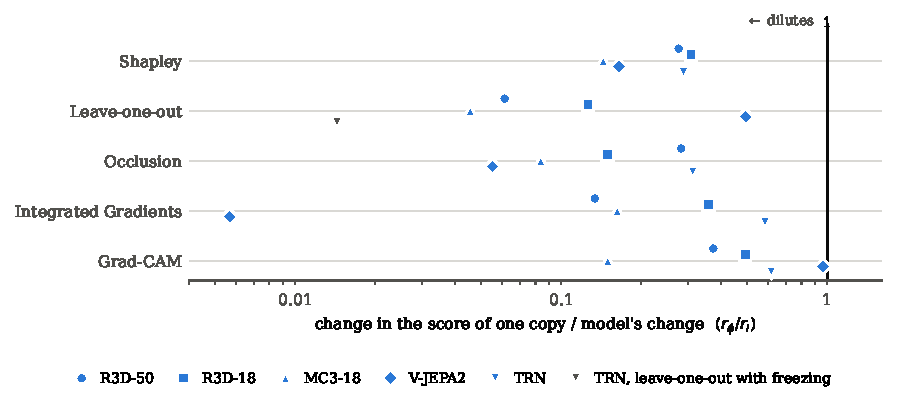
\includegraphics[width=0.85\textwidth]{figures/fig_dilution.pdf}
\caption{How much each attribution method dilutes a repeated frame, under controlled repetition (E1). The change in the score of one copy of the target divided by the model's own change, $r_\phi / r_I$, per target, then the median over targets; 1 means that the score follows the model. Largest number of copies tested (four times the reference on R3D-50 and R3D-18, nine times on MC3-18 and V-JEPA2, two times on TRN); exact copies. Leave-one-out uses deletion except on TRN (grey), where only freezing is possible and part of the result is fixed by the operator (Section~\ref{sec:removal}).}
\label{fig:bias-map}
\end{figure}

Every attribution method dilutes on every model: no point reaches 1.
How much it dilutes depends on the method and the model.
\begin{itemize}
  \item \textbf{Shapley values} keep 0.14--0.31 of the model's change per copy, on all five models.
  \item \textbf{Leave-one-out} keeps 0.05--0.49 with deletion, and 0.01 on TRN with freezing. \textbf{Occlusion} keeps 0.06--0.31.
  \item \textbf{Integrated Gradients} varies most between models: from 0.006 on V-JEPA2 to 0.58 on TRN.
  \item \textbf{Grad-CAM} comes closest to the model, at 0.37--0.96 on four models. On MC3-18, whose dependence on the target triples, it keeps 0.15.
\end{itemize}
These values are medians of per-target ratios, so they differ from the medians of the per-copy scores reported in Table~\ref{tab:e1-loo} and in the E1 report, which are taken separately from the median of $r_I$.
% Source: motivation/fig_dilution.py (prints every plotted value).

\todo{Subsection: Shapley values and Play Fair.}

\subsection{Leave-one-out}
\label{sec:e1-loo}

Leave-one-out depends on the removal operator, and with freezing part of its result is fixed by the operator alone (Section~\ref{sec:why}, Appendix~\ref{app:loo-freeze}).
We therefore report it with deletion wherever the model allows it: on MC3-18 and V-JEPA2, which use deletion throughout, and on R3D-50 and R3D-18, where removing a single frame shortens the clip only from 16 to 15 frames (Section~\ref{sec:removal}).
TRN accepts only 8 frames, so for TRN we can only report leave-one-out with freezing.
Table~\ref{tab:e1-loo} gives both operators for the R3D models, to show how much the operator matters.

\begin{table}[h]
\centering
\caption{Leave-one-out under controlled repetition, at the largest number of copies tested. ``Copies'' is the number of copies of the target relative to the reference clip. $r_I$ is the model's own change in dependence on the target. Score per copy: the mean leave-one-out score of one copy of the target, relative to the reference clip, for the target clip and for the control clip. $\beta$: dilution slope with 95\% bootstrap interval ($\beta = -1$ is an even split among the copies). Medians over targets. Exact copies. Freezing rows for TRN, and for R3D-50 and R3D-18 for comparison, are marked $^\dagger$: their scores are partly fixed by the operator.}
\label{tab:e1-loo}
\begin{tabular}{llccccc}
\toprule
 & & & & \multicolumn{2}{c}{score per copy} & \\
\cmidrule(lr){5-6}
model & removal & copies & $r_I$ & target & control & $\beta$, target (control) \\
\midrule
R3D-50  & deletion & $\times 4$ & 1.28 & 0.01 & 0.64 & $-0.27$ $[-0.72, -0.15]$ ($+0.17$) \\
R3D-18  & deletion & $\times 4$ & 1.30 & 0.36 & 0.56 & $\phantom{-}0.00$ $[-0.26, \phantom{-}0.17]$ ($+0.13$) \\
MC3-18  & deletion & $\times 9$ & 3.22 & 0.13 & 0.70 & $-0.77$ $[-0.84, -0.70]$ ($-0.14$) \\
V-JEPA2 & deletion & $\times 9$ & 0.87 & 0.30 & 0.83 & $-0.48$ $[-0.69, -0.22]$ ($-0.05$) \\
\midrule
TRN     & freezing$^\dagger$ & $\times 2$ & 1.32 & 0.02 & 1.03 & $-2.60$ $[-3.19, -2.25]$ ($+0.25$) \\
R3D-50  & freezing$^\dagger$ & $\times 4$ & 1.28 & $-0.05$ & 0.39 & $-1.38$ $[-1.91, -1.07]$ ($-0.11$) \\
R3D-18  & freezing$^\dagger$ & $\times 4$ & 1.30 & $-0.02$ & 0.62 & $-1.55$ $[-1.69, -1.38]$ ($-0.09$) \\
\bottomrule
\end{tabular}
\end{table}

\paragraph{With deletion, leave-one-out dilutes on every model where it can be tested.}
On all four models, the score of one copy of the target falls well below its value in the control clip, and well below the model's own change in dependence on the target ($r_I$ between 0.87 and 3.22).
How far it falls depends on the model.
On R3D-50, each copy keeps almost none of its score (0.01).
On MC3-18, it keeps 0.13, although the model's dependence on the target more than triples.
On V-JEPA2 and R3D-18, it keeps 0.30 and 0.36.
On R3D-18, 0.36 is close to an even split of the model's dependence among four times as many copies ($1.30 / 4 = 0.33$).
The dilution slope of the target lies clearly below that of its control on MC3-18 and V-JEPA2, where the two intervals do not overlap.
On R3D-50 it is also below, but the interval of the control ($[-0.18, +0.43]$) overlaps that of the target slightly.
On R3D-18, the two intervals overlap on the 120 videos used for the comparison with freezing; on all 345 videos with E1 clips, the slope is $-0.19$ $[-0.31, -0.08]$ for the target and $+0.08$ $[+0.02, +0.18]$ for the control, with 0.44 per copy.

\paragraph{With freezing, the score per copy is close to zero on every model, but this is partly fixed by the operator.}
On R3D-50, deletion gives a similar result (0.01 against $-0.05$ per copy), so there the near-zero score does not come from the operator.
On R3D-18, it does: deletion gives 0.36 per copy and a slope of 0.00, against $-0.02$ and $-1.55$ with freezing.
On TRN, we cannot separate the two.
Its result is consistent with dilution, but part of it may come from the operator, as on R3D-18.

\todo{Subsection: occlusion, Integrated Gradients and Grad-CAM (score per copy, against the model's change and against the control clips).}

\todo{Subsection: rankings (inversions; leave-one-out with deletion on R3D-18: 50\% against 37\% in the control).}


\bibliography{main}
\bibliographystyle{tmlr}

\appendix
% Appendix. Included from main.tex after the references.

\section{Proof of Proposition~\ref{prop:split}}
\label{app:proofs}

% Checked numerically on 300 random games with 3-7 players:
% scratchpad check_prop1.py (exact case: |phi_i - phi_j| = 0; approximate case: ratio <= 0.98).

Write $w(s) = s!\,(n - s - 1)!/n!$ for the weight that the Shapley value gives to a subset of size $s$.
Assume $n \ge 2$.

\paragraph{Step 1: pair the subsets.}
The Shapley value $\phi_i$ sums over all subsets of the other frames, $N \setminus \{i\}$.
Each of these subsets either does not contain $j$, in which case it is some $S \subseteq N \setminus \{i, j\}$, or contains $j$, in which case it is $S \cup \{j\}$ for some $S \subseteq N \setminus \{i, j\}$.
Grouping the two terms that share the same $S$ gives
\begin{equation*}
  \phi_i = \sum_{S \subseteq N \setminus \{i, j\}}
  \Bigl( w(|S|)\,[v(S \cup \{i\}) - v(S)] + w(|S| + 1)\,[v(S \cup \{i, j\}) - v(S \cup \{j\})] \Bigr).
\end{equation*}
Exchanging the roles of $i$ and $j$ gives the same expression for $\phi_j$, with $v(S \cup \{j\})$ in the first bracket and $v(S \cup \{i\})$ subtracted in the second.

\paragraph{Step 2: subtract.}
The terms $v(S)$ and $v(S \cup \{i, j\})$ cancel, and
\begin{equation*}
  \phi_i - \phi_j = \sum_{S \subseteq N \setminus \{i, j\}} \bigl( w(|S|) + w(|S| + 1) \bigr)\,
  \bigl[ v(S \cup \{i\}) - v(S \cup \{j\}) \bigr].
\end{equation*}

\paragraph{Step 3: the weights sum to one.}
There are $\binom{n-2}{s}$ subsets $S$ of size $s$, and
\begin{equation*}
  \binom{n-2}{s} w(s) = \frac{n - s - 1}{n(n-1)}, \qquad
  \binom{n-2}{s} w(s + 1) = \frac{s + 1}{n(n-1)} .
\end{equation*}
Their sum is $1/(n-1)$ for every $s$, so the total weight over $s = 0, \dots, n-2$ is $1$.
The weights are non-negative, so $\phi_i - \phi_j$ is a weighted average of the differences $v(S \cup \{i\}) - v(S \cup \{j\})$.
Each difference lies in $[-\varepsilon, \varepsilon]$, hence $|\phi_i - \phi_j| \le \varepsilon$.

\paragraph{Step 4: the content.}
For $i \in C$,
\begin{equation*}
  \phi_i - \frac{\Phi_C}{m} = \frac{1}{m} \sum_{j \in C} (\phi_i - \phi_j).
\end{equation*}
The term $j = i$ is zero, and each of the other $m - 1$ terms has absolute value at most $\varepsilon$ by Step 3.
So $|\phi_i - \Phi_C / m| \le (m - 1)\,\varepsilon / m$.
With $\varepsilon = 0$, this gives $\phi_i = \Phi_C / m$. \hfill $\square$

\section{Play Fair and Shapley values with deletion}
\label{app:playfair}

% Source: results/E1_report.md section 4.4; results/e1/R3D_E1_summary.md section 6.2;
% results/e1/MC3_18_E1_summary.md. Play Fair: official attributor (run_playfair.py),
% 256 sampled subsets per subset size, 1 seed. Shapley-drop: 64 orderings, seeds 0 and 1.

We ran the authors' Play Fair code on the E1 clips of two models, with the same value function as our Shapley values with deletion (Shapley-drop).
As a measure of sampling noise alone, we compare two runs of Shapley-drop with different random seeds.

\begin{table}[h]
\centering
\caption{Play Fair against Shapley values with deletion (Shapley-drop) on the E1 clips. Correlations are between the frame scores of each clip (median over clips). The last row is the share of clips.}
\label{tab:playfair}
\begin{tabular}{lcc}
\toprule
 & R3D-50 (27 targets) & MC3-18 (32 targets) \\
\midrule
correlation, Play Fair vs.\ Shapley-drop seed 0 & 0.79 & 0.84 \\
correlation, Shapley-drop seed 1 vs.\ seed 0 & 0.65 & 0.78 \\
Play Fair closer to seed 0 than seed 1 is & 91\% & 88\% \\
\bottomrule
\end{tabular}
\end{table}

Play Fair is closer to Shapley-drop than Shapley-drop is to itself, because this run of Play Fair used more model evaluations per clip than one run of Shapley-drop.
For every target, we also compared the per-copy ratio and the dilution slope $\beta$ between Play Fair and Shapley-drop.
All 95\% intervals of the differences include zero, and the differences are about as large as those between the two seeds of Shapley-drop.
MC3-18 is the more informative of the two models, because its output hardly depends on clip length, so deleting frames is valid there (Appendix~\ref{app:length}).
On R3D-50, both methods mix the effect of content with the effect of length, but they still agree with each other.
\todo{Check the number of model evaluations per clip on MC3-18 (about 2,650 for Play Fair against 1,000 for one Shapley-drop seed on R3D-50).}

\section{A reference that averages over subsets}
\label{app:reference}

% Source: results/e1/<model>_group_rows.csv (motivation/e1_group.py, e1_group_metrics.py).
% Exact copies, target clips, largest number of copies. Columns I_t, group_oracle (group_pairs
% on V-JEPA2), frame_per_copy, frame_total. Script: scratchpad cmp2.py.

Importance $I(C)$ measures the drop in output when the content is removed from the full clip only (Section~\ref{sec:problem}).
To check that our conclusions do not depend on this choice, we repeat the comparison with a reference that averages over all subsets of the other frames: the group Shapley value $\Psi_C$ of the content, computed with all frames of the content as one player (Section~\ref{sec:groups}).
Its change is $r_\Psi = \Psi'_{C'} / \Psi_C$.
We use the E1 clips on which group values were computed, with the same removal operator as in the rest of E1.
On V-JEPA2, the other contents are joined into neighbouring pairs so that the group values can be computed exactly.

\begin{table}[h]
\centering
\caption{The model's change measured by importance ($r_I$) and by the group Shapley value ($r_\Psi$), and the frame-level Shapley values of the target compared with each. Exact copies, largest number of copies. Medians over targets, with the interquartile range for $r_I$ and $r_\Psi$. $\rho$: Spearman rank correlation between $r_I$ and $r_\Psi$ across targets. Score per copy: $r_\phi$ divided by the reference named in the column (targets with both references positive).}
\label{tab:reference}
\begin{tabular}{lcccccc}
\toprule
 & & & & & \multicolumn{2}{c}{score per copy} \\
\cmidrule(lr){6-7}
model & targets & $r_I$ & $r_\Psi$ & $\rho$ & $/\,r_I$ & $/\,r_\Psi$ \\
\midrule
R3D-50  & 74  & 0.98 $[0.24, 3.24]$ & 1.09 $[0.88, 1.24]$ & 0.78 & 0.29 & 0.51 \\
R3D-18  & 90  & 1.30 $[0.41, 2.26]$ & 1.06 $[0.94, 1.21]$ & 0.81 & 0.29 & 0.46 \\
MC3-18  & 86  & 2.88 $[1.17, 4.34]$ & 1.02 $[0.11, 1.79]$ & 0.75 & 0.16 & 0.40 \\
V-JEPA2 & 45  & 0.85 $[0.23, 1.11]$ & 0.91 $[0.30, 1.16]$ & 0.72 & 0.22 & 0.24 \\
TRN     & 200 & 1.32 $[0.92, 2.32]$ & 1.12 $[0.97, 1.27]$ & 0.68 & 0.30 & 0.40 \\
\bottomrule
\end{tabular}
\end{table}

Table~\ref{tab:reference} shows three things.
\begin{itemize}
  \item \textbf{The two references agree in their median on four models.} On R3D-50, R3D-18, V-JEPA2 and TRN, the median changes are within 0.25 of each other, and across targets the two are rank-correlated ($\rho$ between 0.68 and 0.81). On R3D-50, R3D-18 and TRN, the group Shapley value varies much less between targets than importance does.
  \item \textbf{They disagree on MC3-18.} Importance says that the model depends on a target shown nine times about 2.9 times as much as before; the group Shapley value stays at about 1.0. Removing all copies from the full clip costs more than before, but averaged over subsets of the other frames the content adds about as much as before.
  \item \textbf{The conclusion holds under both references.} With either reference, the frame-level Shapley score of one copy falls well below the model's change on every model (0.16--0.51), so Shapley values dilute.
\end{itemize}

\section{Every frame shown several times}
\label{app:whole-repeat}

% Source: results/e1/mc3_18_whole_repeat.jsonl and _summary.txt (motivation/whole_clip_repeat.py).
% Shapley run stopped after 20 of 30 videos (GPU memory); its result is exact on all 20.

Proposition~\ref{prop:conflict} gives an exact prediction when the content is the whole clip: an efficient method gives $r_\phi = r_I / m$.
Section~\ref{sec:why} argues that Integrated Gradients does the same on the logit scale, and that Grad-CAM falls by about the factor $m$ through the model's pooling.
We test these predictions on MC3-18, whose output hardly depends on the number of frames (Appendix~\ref{app:length}), so longer clips can be given to it directly.
We take the 16-frame clips of the first 100 E1 videos and show every frame $m = 2$ or $3$ times in a row, which gives clips of 32 and 48 frames, with the predicted class of the original clip.
Shapley values (64 random orderings, deletion) were computed on the first 20 of these videos, because they are costly on 48 frames.
We report $r_\phi / (r_I / m)$, which is 1 when the method dilutes by exactly $m$, and the same ratio with the change in the logit difference $r_F$ in place of $r_I$.

\begin{table}[h]
\centering
\caption{Every frame shown $m$ times, MC3-18. Medians over videos, with the interquartile range. $r_I$: the model's own change, $(v(N') - v(\emptyset)) / (v(N) - v(\emptyset))$. $r_F$: the change in the logit of the class minus its logit on the flat-frame baseline of Integrated Gradients. Videos whose prediction changed, or whose mean score on the original clip is not positive, are left out.}
\label{tab:whole-repeat}
\small
\setlength{\tabcolsep}{4pt}
\begin{tabular}{lcccccc}
\toprule
 & & & \multicolumn{2}{c}{$r_\phi / (r_I / m)$} & \multicolumn{2}{c}{$r_\phi / (r_F / m)$} \\
\cmidrule(lr){4-5} \cmidrule(lr){6-7}
method & videos & $r_I$, $m = 3$ & $m = 2$ & $m = 3$ & $m = 2$ & $m = 3$ \\
\midrule
Shapley values        & 20 & 0.96 & 1.00 $[1.00, 1.00]$ & 1.00 $[1.00, 1.00]$ & 1.01 $[0.99, 1.03]$ & 1.00 $[0.97, 1.03]$ \\
Integrated Gradients  & 97 & 0.94 & 1.01 $[0.97, 1.07]$ & 1.03 $[0.96, 1.10]$ & 1.00 $[0.98, 1.03]$ & 1.01 $[0.97, 1.04]$ \\
Grad-CAM              & 97 & 0.94 & 0.94 $[0.88, 1.00]$ & 0.91 $[0.84, 0.99]$ & 0.92 $[0.88, 0.98]$ & 0.89 $[0.82, 0.96]$ \\
Occlusion             & 95 & 0.94 & 1.03 $[0.91, 1.13]$ & 1.02 $[0.89, 1.16]$ & 1.03 $[0.88, 1.13]$ & 1.01 $[0.84, 1.18]$ \\
\bottomrule
\end{tabular}
\end{table}

\begin{itemize}
  \item \textbf{The model barely changes.} Its own change $r_I$ is 0.94--0.97, so an attribution that follows the model would keep almost all of its score per frame.
  \item \textbf{Shapley values dilute by exactly $m$}, as Proposition~\ref{prop:conflict} states: the ratio is 1.00 on every video.
  \item \textbf{Integrated Gradients dilutes by $m$ on the logit scale} (1.00--1.01), and within a few percent of $m$ on the probability scale.
  \item \textbf{Grad-CAM dilutes by slightly more than $m$} (0.91--0.94), so the division by the model's pooling is close to the factor $m$ even with the ReLU and an intermediate layer.
  \item \textbf{Occlusion also dilutes by about $m$} (1.02--1.03), although no property of its definition forces it to.
  \item \textbf{Leave-one-out is close to zero throughout.} Its mean absolute score per frame is only 0.022 of the output change $v(N) - v(\emptyset)$ on the original clip, because neighbouring frames of a 16-frame clip already stand in for each other, and it falls to 0.011 and 0.008 at $m = 2$ and $3$. Its mean score on the original clip is positive in only 15 videos, too few for a ratio.
\end{itemize}
In all four methods with a usable ratio, sampling every frame $m$ times lowers the score of every frame to about $1/m$ of its value, while the model's dependence on the clip stays almost the same.

\section{Leave-one-out under freezing}
\label{app:loo-freeze}

% Source: results/e1/<model>_attributions.jsonl, method loo_freeze, exact copies, all conditions.

On R3D-50, R3D-18 and TRN, frames are removed by freezing: a removed slot is filled with a kept neighbouring frame, and the output is averaged over a fill from the preceding and from the following kept frame.
Leave-one-out with this operator scores slot $i$ by
\begin{equation}
  \phi_i = v(N) - \tfrac{1}{2}\bigl[ f_c(x^{\leftarrow i}) + f_c(x^{\rightarrow i}) \bigr],
\end{equation}
where $x^{\leftarrow i}$ and $x^{\rightarrow i}$ are the clips in which slot $i$ is replaced by its preceding and following kept frame.
If the neighbour on one side shows the same content as slot $i$, the corresponding filled clip is identical to $x$.
This gives three cases for a slot $i$:
\begin{itemize}
  \item \textbf{interior copy:} both neighbours are copies of the same content. Both filled clips equal $x$, so $\phi_i = 0$ exactly.
  \item \textbf{edge copy:} one neighbour is a copy. One filled clip equals $x$, so $\phi_i$ is half the effect of filling the slot with the other neighbour.
  \item \textbf{single frame:} neither neighbour shows the same content.
\end{itemize}
A \emph{slot} is one position in the clip: R3D-50 and R3D-18 clips have 16 slots, and TRN clips have 8.
Leave-one-out gives one score per slot.
To build Table~\ref{tab:loo-freeze}, we took every E1 clip with exact copies (reference, target and control clips, from all videos), sorted each slot into one of the three cases above, and pooled the slots of each case across all clips.
Each cell gives the median absolute leave-one-out score of the slots in that case, and, in brackets, the number of slots the median is taken over.
For example, R3D-50 has 8{,}560 edge copies across all its clips, and the median of their scores is 0.008.
Every interior copy has a score of exactly zero.
In the reference clips of these models, each content is shown in two adjacent slots (the reallocation design, Section~\ref{sec:adding}), so every copy is an edge copy.
In a target clip with $m$ adjacent copies, at least $m - 2$ of them are interior copies, so the mean score per copy is at most $2/m$ of the edge score.
This accounts for the steep fall of the leave-one-out score per copy as the target is repeated more often on these models (dilution slope $\beta$ between $-2.60$ and $-1.38$, below the value $-1$ of an even split).

\begin{table}[h]
\centering
\caption{Leave-one-out scores with freezing, for slots whose neighbours are copies of the same content on both sides (interior copy), on one side (edge copy), or on neither side (single frame). All E1 clips with exact copies. First row: the share of slots whose score is exactly zero. Other rows: the median absolute score, with the number of slots in brackets. The first and last slot of each clip are left out (see text).}
\label{tab:loo-freeze}
\begin{tabular}{lccc}
\toprule
 & interior copy & edge copy & single frame \\
\midrule
share of scores exactly 0, all models & 1.00 & 0.00--0.01 & 0.00 \\
R3D-50 & 0 (3{,}716) & 0.008 (8{,}560) & 0.019 (3{,}716) \\
R3D-18 & 0 (4{,}508) & 0.008 (9{,}678) & 0.018 (4{,}508) \\
TRN & 0 (808) & 0.018 (2{,}724) & 0.061 (808) \\
\bottomrule
\end{tabular}
\end{table}
A copy in the first or last slot of the clip has only one neighbour, so freezing fills it from that side alone.
If that neighbour is a copy, the filled clip again equals the input.
These slots are left out of the table (1{,}160 on R3D-50, 1{,}306 on R3D-18 and 852 on TRN); 48--53\% of their scores are exactly zero, and the rest are below 0.0015.
% Counts: scratchpad loo_freeze_cells.py on results/e1/<model>_attributions.jsonl (loo_freeze, exact).

The result is not specific to exact copies in principle.
In a natural video, a slot whose neighbours are near-identical frames is filled with a near-identical frame, and its leave-one-out score is close to zero for the same reason.
But in E1, where the copies are exact, the score of an interior copy is zero regardless of the model.
Under deletion, removing a copy shortens the clip, so the input always changes and the score depends on the model.
R3D-50 accepts clips shorter than 16 frames, and E1 also computed leave-one-out with deletion on it.
At four times the reference number of copies, the median score per copy is 0.006 of its reference value with deletion, against 0.64 in the control clips.
With freezing, the same values are $-0.05$ and $0.39$.
So on R3D-50, leave-one-out gives copies almost no credit with either operator; the result does not come from the operator alone.
On MC3-18 and V-JEPA2, which use deletion throughout, the score per copy is 0.13 and 0.30 of its reference value.
On R3D-18 the operator matters much more.
We ran leave-one-out with deletion on the same 120 videos as the E1 run with freezing (R3D-18's accuracy is 82.2\% with 15 frames and 84.4\% with 16).
At four times the reference number of copies, the median score per copy is 0.36 of its reference value with deletion, against $-0.02$ with freezing; in the control clips it is 0.56 and 0.62.
The dilution slope is $0.00$ $[-0.26, 0.17]$ for the target and $+0.13$ $[-0.09, 0.38]$ for the control, against $-1.55$ for the target with freezing.
On all 345 videos with E1 conditions, the slope is $-0.19$ $[-0.31, -0.08]$ for the target and $+0.08$ $[0.02, 0.18]$ for the control.
The model's own dependence on the target rises to 1.30 times its reference value, so a score of 0.36 per copy still falls short of it, but the near-zero score obtained with freezing comes mostly from the operator.
TRN accepts only 8 frames, so deletion is not possible there.
\todo{Rewrite the E1 leave-one-out claim in the results section with these numbers. Source: results/e1/r3d\_18\_attributions.jsonl, method loo\_drop; metrics from e1\_metrics.py on the first 120 videos.}

\section{Occlusion and the response to the flat frame}
\label{app:flat-frame}

% Sources: motivation/occlusion_check.py (single frames, deletion models)
%          motivation/occlusion_all_copies.py (all copies, freeze models)
%          results/e1/<model>_occ_all_copies.jsonl

Occlusion replaces a slot with a flat frame: a frame in which every pixel has the same colour, the average colour that the model's input normalisation subtracts.
For R3D-50, R3D-18 and MC3-18 this is the average colour of Kinetics, the dataset they were pre-trained on; for TRN and V-JEPA2 it is the average colour of ImageNet.
% V-JEPA2: AutoVideoProcessor of facebook/vjepa2-vitl-fpc16-256-ssv2, image_mean (0.485, 0.456, 0.406).
The change in output then has two sources: the loss of the slot's content, and the presence of a frame that does not occur in natural videos.
Only the first is related to redundancy.

\paragraph{Measurement.}
For each content $C$ in an E1 reference clip, we compare two clips that remove the same slots, every slot that shows $C$, in two ways:
\begin{equation}
  \mathrm{occ}(C) = v(N) - f_c(x \text{ with every slot of } C \text{ flat}), \qquad
  I(C) = v(N) - v(N \setminus C).
\end{equation}
$I(C)$ uses the model's removal operator (deletion or freezing), so $D(C) = \mathrm{occ}(C) - I(C)$ is the effect of the flat frame relative to that operator.
On MC3-18 and V-JEPA2 each content is shown in one slot; on R3D-50, R3D-18 and TRN it is shown in two slots, and both are made flat.
The importance $I(C)$ of every content in these clips was already computed when the E1 clips were built.
We compute it again in the same run as $\mathrm{occ}(C)$, from the rebuilt clips, as a check that the clips are rebuilt exactly.
The two agree to within $8 \times 10^{-4}$, except on V-JEPA2, where the first computation used half-precision arithmetic and this one full precision (median difference 0.001).
We focus on contents in the lowest third of $|I(C)|$: removing them barely changes the output, so a large occlusion score must come from the flat frame.

\begin{table}[h]
\centering
\caption{Occlusion of every slot of a content, $\mathrm{occ}(C)$, against the content's importance, $I(C)$. All contents of all E1 reference clips of each model, pooled. Rows 3--4: medians over the contents in the lowest third of $|I(C)|$, which the model barely depends on. Rows 5--6: medians over all contents.}
\label{tab:flat-frame}
\begin{tabular}{lccccc}
\toprule
 & MC3-18 & TRN & R3D-50 & R3D-18 & V-JEPA2 \\
\midrule
removal operator & deletion & freezing & freezing & freezing & deletion \\
videos (contents) & 265 (4{,}240) & 245 (980) & 220 (1{,}760) & 345 (2{,}760) & 34 (544) \\
$|I(C)|$, lowest third & 0.003 & 0.012 & 0.005 & 0.006 & 0.006 \\
$\mathrm{occ}(C)$, lowest third & \textbf{0.020} & \textbf{0.154} & 0.005 & 0.004 & 0.001 \\
$|D(C)|$, all & 0.025 & 0.206 & 0.041 & 0.026 & 0.037 \\
$|I(C)|$, all & 0.010 & 0.112 & 0.025 & 0.024 & 0.031 \\
\bottomrule
\end{tabular}
\end{table}
% All five columns: motivation/occlusion_all_copies.py.

\paragraph{Results.}
On MC3-18 and TRN, the response to the flat frame dominates the occlusion score of unimportant content: occluding it lowers the output by about 7 and 13 times as much as removing it.
On these two models the flat frame also pushes the output in a consistent direction: $D(C) > 0$, meaning that occlusion lowers the output more than removal does, for 93\% of the contents on MC3-18 and 71\% on TRN.

On R3D-50, R3D-18 and V-JEPA2, occlusion and importance have similar medians for unimportant content, but this does not mean that the flat frame has no effect.
It has no consistent direction: $D(C) > 0$ for 63\% of the contents on R3D-50, 57\% on R3D-18 and 49\% on V-JEPA2, and $D(C) < 0$ for the rest.
Positive and negative differences cancel in the median of $D(C)$, but not in the median of $|D(C)|$, which is as large as the median $|I(C)|$ or larger (0.041 against 0.025 on R3D-50, and 0.037 against 0.031 on V-JEPA2).
So occlusion often gives a content a score far from its importance, upwards for some contents and downwards for others.
A consequence is that occlusion and importance put the contents in different orders.
We measure this with the Spearman rank correlation between $\mathrm{occ}(C)$ and $I(C)$ over all contents of a model: each content is ranked once by its occlusion score and once by its importance, and the correlation of the two rankings is computed.
A value of 1 means the two orders are identical, and 0 means they are unrelated.
The rank correlation is 0.31 on R3D-50, 0.57 on R3D-18 and 0.26 on V-JEPA2 (0.57 on MC3-18 and 0.32 on TRN).
% Signs and rank correlations: scratchpad flat_sign.py on results/e1/<model>_occ_all_copies.jsonl.

\paragraph{Consequence for dilution.}
On every model, the occlusion score of a frame contains a part that comes from the flat frame, not from the loss of the frame's content, and this part is unrelated to redundancy.
Occlusion is therefore a less direct test of dilution than leave-one-out with deletion.
The response to the flat frame does not explain the behaviour of occlusion on R3D-50, where the score of the target does not change differently from the score in the control clips when the target is repeated (dilution slope $-0.04$ for the target, $+0.24$ for the control).
We leave that case unexplained.

\section{Clip length and the choice of removal operator}
\label{app:length}

% Sources: results/frame_count_*_summary.csv (T2), results/length_fixed_content_*_summary.csv (T3),
% results/design_choice_report.md. 500 test videos per model.

We ran two checks per model on 500 test videos.
The first samples $T$ frames evenly across each video, for $T$ between 1 and 24 (every value from 1 to 24 on R3D-50; 1 to 18, 20 and 24 on R3D-18 and MC3-18; 1, 2, 4, \dots, 16, 18, 20 and 24 on V-JEPA2; and even values up to 16 on VideoMAE, which accepts at most 16 frames).
Every extra frame is new content, so accuracy should rise smoothly; a sudden jump points to the architecture.
The second takes the $k$ frames that the first check uses for $T = k$, and shows them in two ways: as a clip of $k$ frames, and as a clip of 16 frames in which each frame is repeated several times in a row, in its original order. When 16 is not a multiple of $k$, some frames are repeated once more than others; for example, with $k = 3$ the frames are repeated 6, 5 and 5 times.
We use every $k$ from 1 to 16 on R3D-50; $k = 1, 2, 4, 6, \dots, 16$ on R3D-18, MC3-18 and V-JEPA2; and even $k$ from 2 to 16 on VideoMAE, which processes frames in pairs.
At $k = 16$ the two clips are identical, so this value is the reference.
The two clips differ in length and in whether frames are repeated, so we read them together with the original clip ($k = 16$), as described in Section~\ref{sec:removal}.
For example, on R3D-50 with $k = 4$, the clip with repeated frames reaches 78.4\%, close to the original's 79.4\%, while the short clip reaches 25.6\%: the loss comes from the length.
On VideoMAE with $k = 8$, the clip with repeated frames reaches 45.6\% and the short clip 66.4\%: the loss comes from the repetition.
On V-JEPA2, both clips lose accuracy together as $k$ falls (47.2\% and 50.4\% at $k = 4$, against 68.2\% for the original): the loss comes from having fewer distinct frames.

\begin{table}[h]
\centering
\caption{Accuracy (\%) with $T$ frames sampled evenly from the video. -- : not tested.}
\label{tab:length-t2}
\setlength{\tabcolsep}{4pt}
\begin{tabular}{lcccccccccccc}
\toprule
$T$ & 3 & 4 & 5 & 8 & 9 & 10 & 14 & 15 & 16 & 17 & 18 & 24 \\
\midrule
R3D-50  & 24.8 & 25.6 & 31.8 & 36.4 & 64.8 & 66.8 & 74.4 & 77.0 & 79.4 & 69.2 & 68.4 & 66.4 \\
R3D-18  & 58.8 & 63.0 & 75.8 & 74.6 & 80.8 & 82.4 & 83.6 & 82.2 & 84.4 & 79.8 & 81.8 & 82.0 \\
MC3-18  & 86.6 & 86.8 & 87.0 & 87.2 & 87.6 & 87.2 & 87.8 & 87.8 & 88.0 & 87.8 & 88.6 & 88.2 \\
V-JEPA2 & --   & 47.2 & --   & 64.6 & --   & 66.8 & 69.0 & 67.2 & 68.2 & --   & 68.4 & 67.8 \\
\bottomrule
\end{tabular}
\end{table}

\begin{table}[h]
\centering
\caption{Accuracy (\%) with the same $k$ distinct frames, shown as a clip of $k$ frames (short) and as a clip of 16 frames in which each frame is repeated several times in a row (repeated). At $k = 16$ both are the original clip. -- : not tested.}
\label{tab:length-t3}
\begin{tabular}{llccccccc}
\toprule
 & $k$ & 1 & 2 & 4 & 6 & 8 & 12 & 16 \\
\midrule
R3D-50   & short    & 15.6 & 17.4 & 25.6 & 35.0 & 36.4 & 71.8 & 79.4 \\
         & repeated & 63.8 & 72.8 & 78.4 & 77.6 & 77.6 & 79.8 & 79.4 \\
\midrule
R3D-18   & short    & 37.8 & 52.0 & 63.0 & 76.2 & 74.6 & 81.6 & 84.4 \\
         & repeated & 67.8 & 75.4 & 81.4 & 82.4 & 81.8 & 83.4 & 84.4 \\
\midrule
MC3-18   & short    & 78.2 & 85.4 & 86.8 & 87.0 & 87.2 & 87.6 & 88.0 \\
         & repeated & 78.6 & 85.0 & 86.4 & 87.2 & 87.2 & 87.2 & 88.0 \\
\midrule
V-JEPA2  & short    & 12.2 & 26.0 & 47.2 & 57.0 & 64.6 & 67.6 & 68.2 \\
         & repeated & 14.4 & 24.4 & 50.4 & 60.8 & 62.4 & 68.6 & 68.2 \\
\midrule
VideoMAE & short    & --   & 42.4 & 56.2 & 63.2 & 66.4 & 73.6 & 76.0 \\
         & repeated & --   & 40.4 & 43.0 & 53.4 & 45.6 & 66.8 & 76.0 \\
\bottomrule
\end{tabular}
\end{table}

\paragraph{What the checks show.}
\begin{itemize}
  \item \textbf{R3D-50 and R3D-18} depend strongly on length. With the same frames, short clips are much less accurate than the same frames repeated to 16 slots: by 41--55 points on R3D-50 for 8 or fewer frames, and by up to 30 points on R3D-18. Accuracy also falls when the clip is longer than 16 frames. Deletion would mix the effect of length with the effect of content, so these models use freezing. Between 15 and 16 frames the difference is 2.4 points on R3D-50 and 2.2 points on R3D-18, small enough for leave-one-out with deletion, which only ever removes one frame.
  \item \textbf{MC3-18} hardly depends on length: the two ways of showing the same frames differ by at most 0.4 points. It uses deletion.
  \item \textbf{V-JEPA2} also hardly depends on length: the two differ by at most 3.8 points, in both directions. It uses deletion.
  \item \textbf{TRN} accepts exactly 8 frames, so it uses freezing.
  \item \textbf{VideoMAE} is less accurate when frames are repeated, by up to 20.8 points (8 frames repeated to 16). It processes frames in pairs, and a pair of identical frames changes its output whatever the frames show. Repeating a frame therefore changes the model's behaviour, so we do not use VideoMAE.
\end{itemize}


\end{document}
